\documentclass[]{article}

\usepackage{natbib}
\bibliographystyle{abbrvnat}
\setcitestyle{authoryear,open={(},close={)}}
\usepackage{pdflscape}
\usepackage{xcolor}
\usepackage{relsize}
\usepackage{listings}
\usepackage{verbatim}
\usepackage{graphicx}
\usepackage{hyperref}
\hypersetup{colorlinks=true}
%\usepackage{mathtools}
\usepackage{amsmath}
\usepackage{float}
%\usepackage{showframe}
\usepackage{placeins}
\usepackage{titlesec}
\setcounter{secnumdepth}{4}
\usepackage{authblk}
\usepackage{longtable}

\titleformat{\paragraph}
{\normalfont\normalsize\bfseries}{\theparagraph}{1em}{}
\titlespacing*{\paragraph}
{0pt}{3.25ex plus 1ex minus .2ex}{1.5ex plus .2ex}


\title{\textbf{\textcolor{blue}{Bayesian Integrated analysis of
      multiple types of rare variants to infer risk genes for
      schizophrenia and other neurodevelopmental disorders}}}

\author[1]{Hoang T Nguyen}
\author[1,2]{Douglas M Ruderfer}
\author[3,4]{Gulio Genovese}
\author[1,5]{Menachem Fromer}
\author[1,3]{Pamela Sklar}
\author[6]{Xin He}
\author[7,8]{Patrick F Sullivan}
\author[1,3,9]{Shaun M Purcell}
\author[1,3]{Eli A Stahl\thanks{eli.stahl@mssm.edu} }
\affil[1]{Division of Psychiatric Genomics, Department of Genetics and Genomic Sciences, Institute for Genomics and Multiscale Biology, Icahn School of Medicine at Mount Sinai, New York, New York 10029, USA}
\affil[2]{Vanderbilt}
 \affil[3]{Stanley Center for Psychiatric Research, Broad Institute of MIT
 and Harvard, Cambridge, Massachusetts, USA.}
 \affil[4]{Department of Genetics, Harvard Medical School, Massachusetts, USA.}
\affil[5]{Verily Life Sciences}
 \affil[6]{Department of Human Genetics, University of Chicago, Chicago, IL
 60637, USA.}
 \affil[7]{Departments of Genetics and Psychiatry, University of North
Carolina, Chapel Hill, North Carolina 27599-7264, USA.}
\affil[8]{Karolinska Instituet}
\affil[9]{Sleep Center, Brigham and Women's Hospital, Harvard Medical School, Boston, Massachusetts, USA.}

\begin{document}
\maketitle

\begin{abstract}
Integrating rare variation from family and case/control studies has
successfully implicated specific genes contributing to risk of autism
spectrum disorder (ASD). In schizophrenia (SCZ), however, while sets of
genes have been implicated through study of rare variation, very few
individual risk genes have been identified. Here, we apply
hierarchical Bayesian modeling of rare variation in schizophrenia and
describe the proportion of risk genes and distribution of risk variant
effect sizes across multiple variant annotation categories. Briefly,
we developed a pipeline based on the previous work used in ASD studies to jointly estimate genetic parameters for one
or multiple combined populations of any disease.
 We applied this method to the largest available collection for rare
variants in schizophrenia (1,077 families, 6,699 cases and 13,028 controls). We defined five variant annotation categories:
disruptive (nonsense, frameshift, essential splice site mutations),
damaging (predicting damaging by seven algorithms), silentCFPK (silent
mutations within frontal cortex-derived DHS)
de novo mutations, and
disruptive and damaging missense case/control singletons. We estimated
that 8.01$\%$ of approximately 20,000 genes are risk genes (95$\%$ credible
interval, CI, 4.59-12.9$\%$), with mean effect sizes (95$\%$ CIs) of 12.25
(4.8- 22.22) for disruptive de novos, 1.44 (1-3.16) for missense
damaging de novos, and 1.22 (1-2.16) for silentCFPK de novos. The mean effect sizes of damaging and disruptive singleton variants for three case-control populations were
2.09 (1.04-3.54), 2.44 (1.04, 5.73) and 1.04 (1-1.19)
respectively. Our analysis identified only two known SCZ risk genes with FDR$<$0.05:
SETD1A and TAF13; and two other genes with FDR $<$ 0.1:  RB1CC1 and
PRRC2A. We further used FDR to analyze the enrichment of several candidate gene
sets. Significant results are observed in gene sets previously
implicated in schizophrenia (including in a subset of these data):
FMRP targets, promoter targets of CHD8, splice
targets of RBFOX, constrained genes, genes with de novo mutations in ASD and
developmental disorder, synaptic genes (need to describe some
'abnormal' genes). Novel result was observed for essential genes which
were found significantly with autism genes in a recent study.
We also applied the pipeline to infer genetic
parameters for a total of 10,792 families and 4,058 cases/controls of four other
neurodevelopmental disorders: autism spectrum disorder (ASD),
intellectual disorder (ID), developmental disorder (DD) and epilepsy
(EPI). The predicted proportions of risk genes in these diseases were smaller
than that in SCZ ($< 5\%$ for all diseases), and larger in ASD ($5\%$) than in the other disorders ($< x\%$).
We report 164 and 58 genes with FDR $<$ 0.05 for DD
and ID, respectively. Of these, 101 of 161 and 15 of 58 genes are not currently
known DD and ID genes.
Overall, our results in schizophrenia
replicate those of previous studies, confirming the robustness of our approach. Our method is able
to identify novel risk genes for SCZ as well as for other diseases.
We conduct power analyses under our inferred model to quantify the improvement in power to detect risk
genes as more data become available.

\end{abstract}

\tableofcontents

\section{Introduction}

Schizophrenia (SCZ) is a complex psychiatric disorder particularly characterized by psychosis, and by positive, negative and cognitive symptoms, with severe medical and social-functioning comorbidities and high public health costs. Despite high
reduction of reproductive fecundity and a lifetime risk of $0.7\%$,
a very high heritability of 60-80$\%$ has been observed for the
disease \citep{lichtenstein2009common, sullivan2003schizophrenia}. The genetic architecture of SCZ is
highly polygenic with the contribution of common, rare and denovo
variants \citep{purcell2014polygenic, fromer2014novo, singh2016rare,  stefansson2009common,purcell2009common}. With the production of
high-quality next-generation sequencing data, the genetics of
schizophrenia and other diseases can be increasingly better characterized, especially for rarer variants.



Rare variants in case/control samples and de novo mutations have been successfully leveraged to
identify specific SCZ risk genes \citep{singh2016rare,takata2016novo}, or to implicate gene sets for this
disease \citep{purcell2014polygenic,fromer2014novo}.
However, the genetic architecture of SCZ for rare variants and de novo mutations has not been inferred. Such analyses could help gain further insight into this disease, for example by using the estimated number of risk genes to calibrate gene discovery false discovery rates, or by using the distribution of effect sizes to estimate power for rare variant association studies. A better understanding of our certainty in sets of risk genes for SCZ will result in a
better picture of biological pathways specific for the disease.

Here, we aim to develop a pipeline for integrative analysis of case-control
rare variants and de novo mutations in order to infer genetic
architecture and identify risk genes
for SCZ as well as other diseases. To do this, we extend a hierarchical model Bayesian analysis framework
(TADA, Transmission And De novo Association) which was developed for
autism spectrum disorder (ASD) \citep{he2013integrated}. The new
framework (\texttt{extTADA}, \underline{ext}ended \underline{T}ransmission \underline{A}nd \underline{D}e novo \underline{A}ssociation) can
be used to analyze only de novo data, only case-control data or the
combination of both.
\texttt{extTADA} uses all variant classes to
simultaneously estimate genetic parameters (therefore it assumes that all classes play important roles in the genetic architecture of the tested disease). In \texttt{extTADA}, a conditional
model for case-control sample frequency allows rapid analysis without population frequency parameters (which are very poorly estimated for rare variants), facilitating estimation of
parameters via Markov Chain Monte Carlo
(MCMC). In addition, we designed \texttt{extTADA} for the analysis of data from multiple population samples.

In this study, we used \texttt{extTADA} to analyze the largest available exome-sequence dataset, including
19,727 (6,699+13,028) case+control samples and 1,077 trio/quad families for SCZ. We estimated mean relative risks (RRs) of different variant annotation categories as
well the proportion of risk genes for disease. Based on these meta-analysis, the false discovery rate (FDR) information of all genes was used to calculate the enrichment of known gene sets and novel gene sets. Analysis of separate classes of variants/mutations in terms of annotation and rarity helps provide a detailed picture of the disease's rare variant genetic architecture.
Finally, we used available data for other neurodevelopmental diseases: intellectual
disability (ID), autism spectrum disorder (ASD), epilepsy (EPI) and
developmental disorder (DD), totaling 10,792 trios
and 4058 cases/controls. We are able to identify additional new
significant genes for ID and DD based on \texttt{extTADA} results.

The pipeline is publicly available at https://github.com/hoangtn/extTADA.

%%%%%%%%%%%%%%
\section{Results}

The \texttt{extTADA} pipeline and its comparison with
\texttt{TADA} is described in Figure \ref{fig:TADAandextTADA}. Figure
\ref{fig:wholedataAnalysis} summarises the workflow of the
current study. As presented in  Figure \ref{fig:wholedataAnalysis},
variants/mutations in this study were divided into categories:
synonymous, missense, loss-of-function (LoF), missense damaging (MiD), silent mutations
within frontal cortex-derived DHS (silentCFPK), and
then three main categories were used in the analysis: MiD, loF and
silentCFPK.

\subsection{\texttt{extTADA} pipeline}

We used an integrated approach in which de novo (DN) and case control (CC)
information was used to infer risk genes. The current study is a
framework which is extended from the Transmission and Disequilibrium
Association (TADA) model proposed by
\cite{he2013integrated, de2014synaptic}. The extensions to
the TADA package consisted of: using an approximate model to estimate parameters
for case-control model, estimating all parameters simultaneously,
controlling the proportion of protective variants and especially using
the model in data sets from multiple populations as shown in Figure \ref{fig:TADAandextTADA}. We used the same
symbols for parameters as those used in \cite{he2013integrated, de2014synaptic} in the following
sections. For completeness, in this section and the Methods section, we also described in detail methods originally presented in the TADA papers \citep{he2013integrated,de2014synaptic}.


In summary, for a given gene, all variants of a category
(e.g., LoF, MiD) were collapsed and considered as a
single count. Let $q$, $\gamma$ and $\mu$ be the population frequency of
genotype (for case/control or transmitted/nontransmitted data),
relative risk (RR) of variants associated with the disease, and
mutation rates of de novo mutations respectively.
At each gene, two hypotheses $H_0:
  \gamma = 1$ and $H_1: \gamma \neq 1$ were compared. A fraction of the genes $\pi$, assumed to be risk genes, were represented by the $H_1$ model. Under this model, relative
  risks ($\gamma$) were assumed to follow a probability distribution.
The model $H_0$ described non-risk genes, and relative risks ($\gamma$)
  of genes were set to equal 1. As in
  \cite{he2013integrated}, we modeled de novo ($x_d$) and case
  ($x_{ca}$) control ($x_{cn}$) data as Poisson distributions and
  their hyper parameters as Gamma distributions. In addition, we
  used Gamma distributions as priors for hyper parameters, a Beta
  distribution to constrain $\pi$ to less than 0.5, and a
  nonlinear function to constrain mean RRs and their variances as described in Table
  \ref{tab:ParameterModelleing}.


\begin{table}[H]
\[
\begin{array}{|l|l|l|}
\hline
 & & \\
x_{dn} \sim P(2N_{dn}\mu  \gamma_{dn}) & \gamma_{dn} \sim
                                         Gamma(\bar{\gamma}_{dn}*\beta_{dn},\beta_{dn})
  & \bar{\gamma}_{dn} \sim Gamma(\bar{\bar{\gamma}}_{dn}, \bar{\beta}_{dn}) \\
& & \beta_{dn} = e^{a*\bar{\gamma}_{dn}^b + c} \\

\hline
& & \\
x_{ca} \sim P(N_{1} q  \gamma_{cc}) & \gamma_{cc} \sim
                                      Gamma(\bar{\gamma}_{cc}*\beta_{cc},
                                      \beta_{cc})
& \bar{\gamma}_{cc} \sim Gamma(\bar{\bar{\gamma}}_{cc}, \bar{\beta}_{cc}) \\
& & \beta_{cc} = e^{a*\bar{\gamma}_{cc}^b + c} \\

& q \sim Gamma(\rho, \nu) & \frac{\rho}{\nu} = mean(\sum(x_{cn} + x_{ca})) \\
& &                    \nu  = 200 \\

\hline
x_{cn} \sim P(N_{0} q) & q \sim Gamma(\rho, \nu)  & \frac{\rho}{\nu} =
                                                    mean(\sum(x_{cn} +
                                                    x_{ca})) \\
& & \nu = 200 \\
\hline
\pi \sim~ Beta(1, 5) &  & \\
\hline
\end{array}
\]

\caption{Parameter information used in all analyses. $N_{dn}, N_1,
  N_0$} are sample sizes of families, cases and controls
respectively. $\bar{\gamma}$ is mean RRs and $\beta$ controls the
dispersion of $\bar{\gamma}$. $\bar{\bar{\gamma}}$ and $\bar{\bar{\beta}}$ are
priors for $\bar{\gamma}$ and are set in advance (they are inferred
from simulation data). $\beta$ is inferred
from the equation $ e^{a*\bar{\gamma}^b + c}$ inside the
estimation process with  a = 6.83, b =
-1.29 and c = -0.58.
\label{tab:ParameterModelleing}
\end{table}



At each gene, a Bayes Factor (BF) was calculated for each category to
compare models $H_1$ and $H_0$ ($BF=P(data|H_1)/P(data|H_0)$). If
there were multiple categories, then $BF_{gene}$ was the product of BFs
for all categories. Data could be from different populations; therefore,
we extended the $BF_{gene}$ for multiple populations as the product of
BFs of all populations as in Equation \ref{eq:bayesfactorAllPops1}. To infer significant genes, BFs were converted to false discovery
rates (FDRs) using the approach in \cite{newton2004detecting}.


\begin{equation} \label{eq:bayesfactorAllPops1}
BF_{gene} = \left[ \prod \limits_{h=1}^{Ndn_{pop}} (\prod \limits_{k=1}^{Cdn}
  BF_{dn_{hk}}) \right]
\left[ (\prod \limits_{a=1}^{Ncc_{pop}} \prod \limits_{b=1}^{Ccc}
  BF_{cc_{ab}}) \right]
\end{equation}

in which: $Ndn_{pop}, Ncc_{pop}$ are the number of populations of DN
and CC data respectively; $C_{dn}, C_{cc}$ are the number of
categories of DN and CC data in that order.

To calculate BFs in Equation \ref{eq:bayesfactorAllPops1}, hyper
parameters of different populations, and categories (assuming $\phi_1$ and $\phi_0$ for $H_1$
and $H_0$ respectively)  in Table
\ref{tab:ParameterModelleing} were needed in advance. Therefore, they
were estimated simultaneously based on a mixture model of two
hypotheses as in Equation \ref{eq:internalModel22}.

\begin{equation}
\label{eq:internalModel22}
\begin{array}{l}
P(x|\phi_1, \phi_0)  = \prod \limits_{i=1}^{Gene\; numbers} \left[ \pi P_{1i} +
 (1 -                  \pi) P_{0i} \right] \\
\end{array}
\end{equation}

where $P_{1i}$ and $P_{0i}$ at the $i^{th}$ gene were calculated across populations and
categories as follows:


\[
\begin{array}{ll}
P_{1i} & = P_{1i}(x_i|\phi_1) \\
& = \left[ P_{1i(dn)}(x_{i(dn)}|\phi_{1(dn)}) \right] \left[
  P_{1i(cc)}(x_{_i(ca)}, x_{i(cn)}|\phi_{1(cc)}) \right] \\
& = \left( \prod \limits_{h=1}^{Ndn_{pop}}
                      \prod \limits_{k=1}^{Cdn} P_{1i(dn)_{hk}}(x_{i(dn)_{hk}}|\phi_{1(dn)_{hk}}) \right)
                      \left( \prod \limits_{a=1}^{Ncc_{pop}}
                      \prod \limits_{b=1}^{Ccc} P_{1i(cc)_{ab}}(x_{i(ca)_{ab}},x_{i(cn)_{ab}}|\phi_{1(cc)_{ab}})
  \right) \\
P_{0i} & = P_{0i}(x_i|\phi_0) \\
& = \left[ P_{0i(dn)}(x_{i(dn)}|\phi_{0(dn)}) \right] \left[
  P_{0i(cc)}(x_{_i(ca)}, x_{i(cn)}|\phi_{0(cc)}) \right] \\
& = \left( \prod \limits_{h=1}^{Ndn_{pop}}
                      \prod \limits_{k=1}^{Cdn} P_{0i(dn)_{hk}}(x_{i(dn)_{hk}}|\phi_{0(dn)_{hk}}) \right)
                      \left( \prod \limits_{a=1}^{Ncc_{pop}}
                      \prod \limits_{b=1}^{Ccc} P_{0i(cc)_{ab}}(x_{i(ca)_{ab}},x_{i(cn)_{ab}}|\phi_{0(cc)_{ab}})
  \right) \\

\end{array}
\]




To simplify the estimation process in Equation
\ref{eq:internalModel22}, we approximated the original model $P(x_{ca}, x_{cn}|H_j)$
using a new model in which case counts were conditioned on total counts:
$P(x_{ca}|x_{ca} + x_{cn})$ (Figure
\ref{fig:TADAandextTADA}). A Markov Chain
Monte Carlo (MCMC) method was used to sample parameters. We extracted
samples from the MCMC process and used their modes for all analyses.
In addition, all credible intervals (CIs) of $5\%$ and $95\%$ were
also used in the inferences of parameters.

\subsection{Test \texttt{extTADA} on simulated data. }

We simulated data for three
situations: one CC category, two CC categories, and one CC category and
one DN category. For CC data, the original TADA model was used to
simulate data, and then the CC approximate
model was used in the estimation process.


\subsubsection{Test \texttt{extTADA} for only CC data}

To test the approximate CC model for
different parameter values, we simulated two situations: one CC class
and two CC classes. We tested on different sample sizes in order to
evaluate the performance of the approximate model.

Overall, high correlations ($\sim 1$) were observed for both situations (Figure
\ref{tab:CorrelationOneClassCC} and
\ref{tab:CorrelationTwoClassCC}). For sample sizes $>$ 3000 cases,
good estimation was observed, but slight over estimation was
observed for the sample size of 1092, especially for risk-gene
proportions.

An additional analysis was carried out to assess the
performance of specific simulated values. Correlations were
calculated for each mean RR and $\pi$ value.
For one CC class, mean RRs were estimated well by
the model with correlations $\sim$ 1 (Figure \ref{fig:CCsimulatedDataDetailed}). However, the proportion of risk
genes was affected by mean RRs. They were estimated well when mean
RRs were between 1.5 and 3.5, but underestimated with smaller mean RRs and
slightly overestimated with larger mean RRs (Figure
\ref{fig:CCsimulatedDataDetailed}). For two CC classes, high
correlations ($\ge 0.97$) between simulated and estimated values were
seen for all parameters. In
addition, small mean RRs of a given class did not directly affect the
estimated values of proportions of risk genes (Figure \ref{fig:2CCsimulatedData}).

The issue of poor estimation for one class, but good estimation
for $>$ one class was expected. This was an advantage of using
multiple classes compared to using only one class in the estimation
process when the clustering signal was not very strong.  Small mean RRs could result in difficulties in the calculation
process to differentiate between a risk gene (mean RR $> 1$) and a
non-risk gene (mean RR $\sim$ 1). If one class was used
then many risk genes would be considered to be non-risk genes. If more
than one class was used, such risk genes would be assigned as genuine
risk genes due to the information available from other classes.



\begin{figure}[ht]
\centering
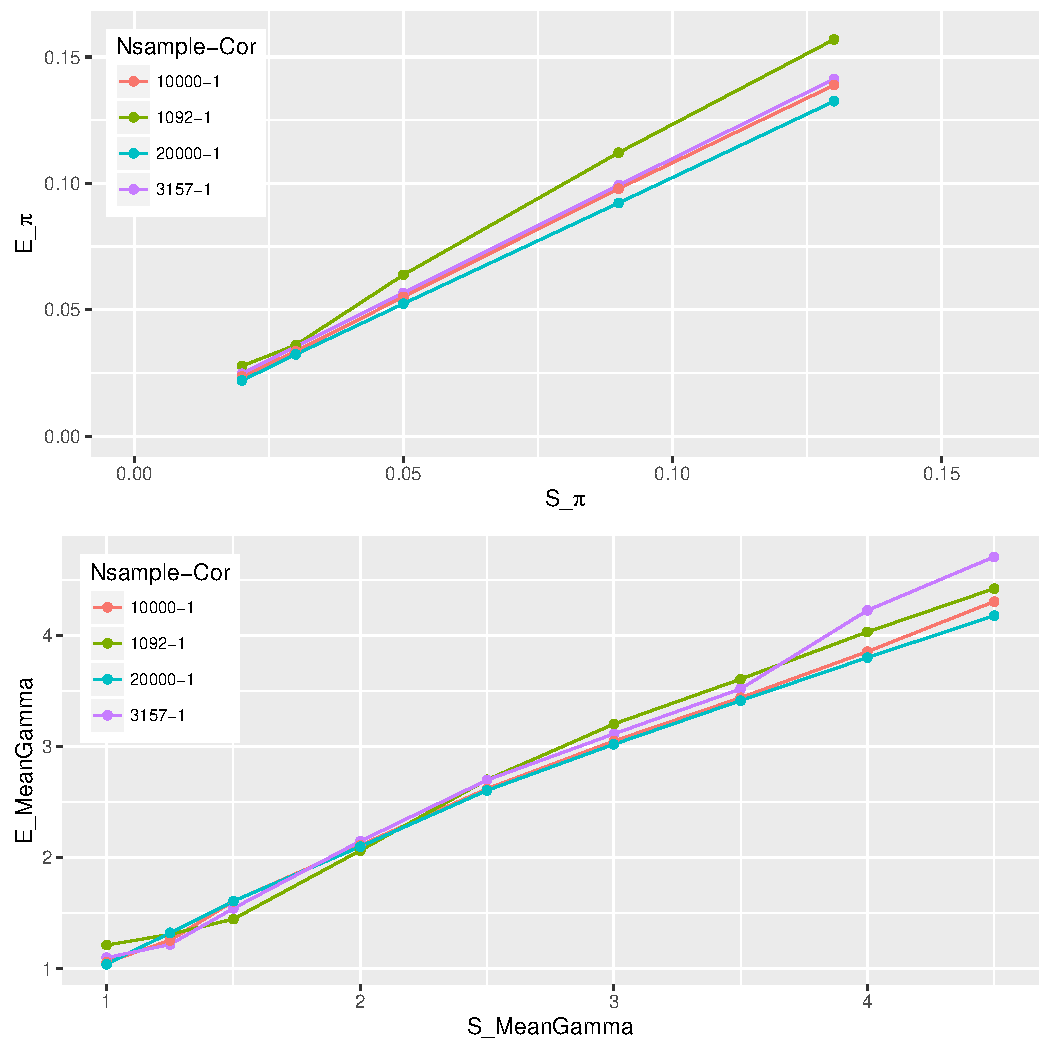
\includegraphics[width=\textwidth,height=8cm]{Picture/PUBOnlyCCnSample.pdf}
\caption{Correlations between estimated and simulated values for one
  CC class with different sample sizes.  X and Y axes describe simulated (S) and estimated (E)
  values respectively. The top picture is for mean relative risks
  (MeanRRs) while the bottom picture is for the proportion of risk
  genes ($\pi$). Legends show sample sizes and correlations.}
\label{tab:CorrelationOneClassCC}
\end{figure}


\begin{figure}[ht]
\centering
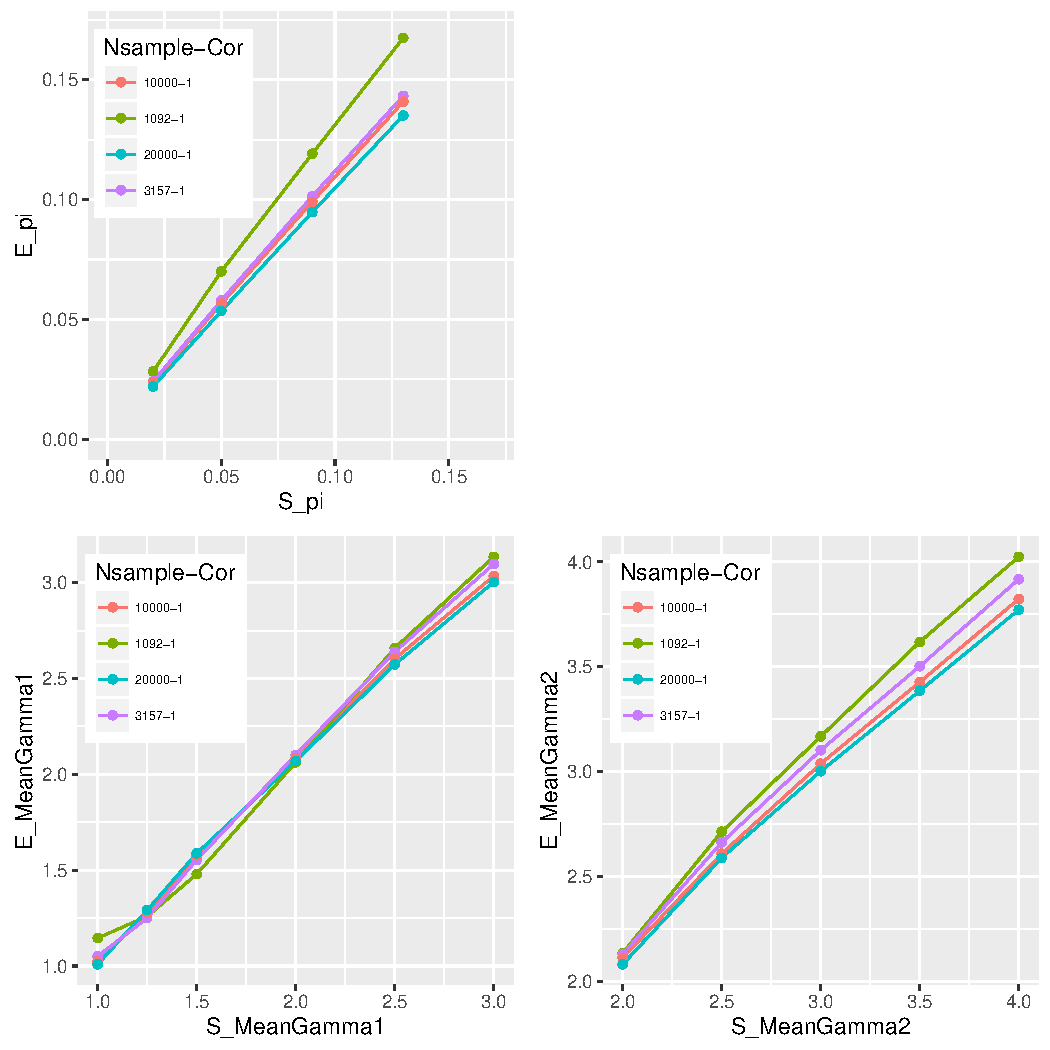
\includegraphics[width=\textwidth,height=8cm]{Picture/PUB2OnlyCCnSample.pdf}
\caption{Correlations between estimated and simulated values for two
  CC class with different sample sizes.  X and Y axes describe simulated (S) and estimated (E)
  values respectively. A range of mean relative risks for two classes
  (MeanRR1 and MeanRRs) and risk-gene proportions ($\pi$) were used in
  the simulation process.  Legends show sample sizes and correlations.}
\label{tab:CorrelationTwoClassCC}
\end{figure}

\subsubsection{Evaluate the performance on integrated DN and CC data}

We next evaluated the main model used in this study as described in Equation
\ref{eq:internalModel22} by combining different values of DN and CC data.
We calculated the ratio of simulated risk genes inside the gene
sets determined with different FDR thresholds. These values were
called observed FDR (oFDR, see the Methods). Overall, high
correlations were observed between FDRs and oFDRs (Figure
\ref{fig:TPRandFPRforDNandCConeClass}). For high $\pi$ values, oFDRs
and FDRs were nearly equal. For small $\pi$ values (e.g., $\pi$ =
0.02) oFDRs were higher than FDRs when mean RRs of de novo data were
small. In addition, oFDRs were equal to zero for many cases when
FDRs were small (Figure \ref{fig:TPRandFPRforDNandCConeClass}). The reason for this was because there were only a few
significant genes with small $\pi$ values and small mean
RRs.


Further investigation into estimated and simulated values was also
carried out. We saw high correlations between estimated and simulated
values (Table \ref{tab:SimulatedParameterOfDNandCC}).
Slightly over and under estimation were observed for mean RRs and
proportions of risk genes. This was
expected and usually did not have a large effect on the final results as discussed
in the previous work \citep{he2013integrated} as well as shown in TPRs
and FPRs results above (Figure \ref{fig:TPRandFPRforDNandCConeClass}).

\begin{figure}[ht]
\centering
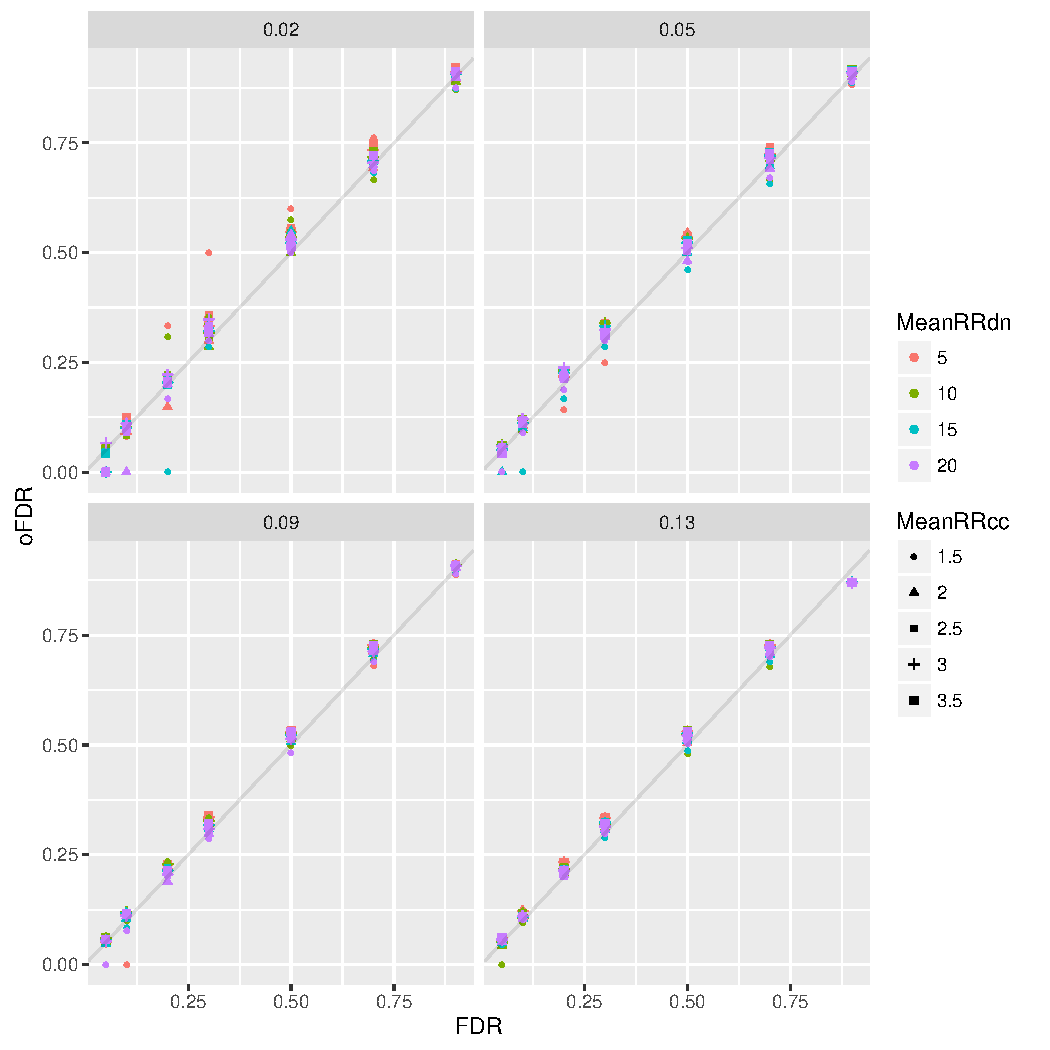
\includegraphics[width=\textwidth,height=8cm]{Picture/FDRandcFDRforDNandCC.pdf}
\caption{Observed false discovery rates (oFDR) with different FDR
  thresholds for different $\pi$ values (0.02, 0.05, 0.09 and 0.13). }
\label{fig:TPRandFPRforDNandCConeClass}
\end{figure}

\FloatBarrier
\subsection{Schizophrenia data sets}

The SCZ data sets were refined into non heterogeneous populations and then
\texttt{extTADA} was used to integratively analyze. The CC data were
also separated into variants present/absent in the  Exome Aggregation Consortium
(ExAC) \citep{lek2015analysis}, termed InExAC and NotExAC respectively. In
total, there were 6,699 cases, 13,028 controls, 1077 trio/quad
families used in this analysis. In addition, we used 731 families
including uninfected siblings as controls for de novo data (Table
\ref{tab:alldata}, Figure \ref{fig:wholedataAnalysis}).

\subsubsection{Extract data sets to analyze integratively}

De novo mutations and case-control variants were tested to select
classes and samples for the meta analysis of the \texttt{extTADA} pipeline.
For case-control data, there were multiple populations and the data
were also sequenced from different centers. Therefore, we classified
the data as follows. Firstly for the 4,929 cases and 6,232 controls of
the Sweden population, we clustered all
cases and controls into different groups and then calculated p values
(using the \emph{lm, glm} function in R) between cases and controls by adjusting and not adjusting
for covariates. We aimed to obtain populations for which results
would not be much different when using or excluding covariates.
We chose a clustering
process that resulted in highly similar results when either incorporating or excluding covariates. The clustering process divided the data set into
three groups as in Figure \ref{fig:homegeneouspopfrompca}: Group 1 =
3,157 cases + 4,672 controls; Group 2 = 681 cases + 367 controls;
and Group 3 = 1,091 cases + 1,193 controls. Only Groups 1 and 3 were
used in the next stage because Group 2 showed a large difference between the
two sets of adjusted and unadjusted results. In addition,
similar to \cite{genovese2016increased}, InExAC variants did
not show significant differences between cases and controls but NoExAC
variants showed some significant differences (Figure
\ref{fig:homegeneouspopfrompca}). Secondly, from the data of the UK10K project \citep{singh2016rare},
only case-control data from the UK population was used. Because high
significance was observed for NoExAC variants, we therefore used only NoExAC
variants in all main analyses. However, we also used both InExAC and
NoExAC variants to form a better picture of the genetic architecture
of the disease in a comparison section.


For de novo mutations, we calculated the sample-adjusted ratios of mutation counts
between 1,077 cases and 731 controls. Similar to
\cite{takata2016novo}, the highest ratio was observed for silentCFPK (2.57),
followed by MiD (2.3), LoF (1.83) and missense, silent ( $\sim $ 1.3)
mutations (Figure \ref{tab:denovomutation}). Three
classes (LoF, silentCFPK, and MiD) were used in next steps.

\begin{figure}[ht]
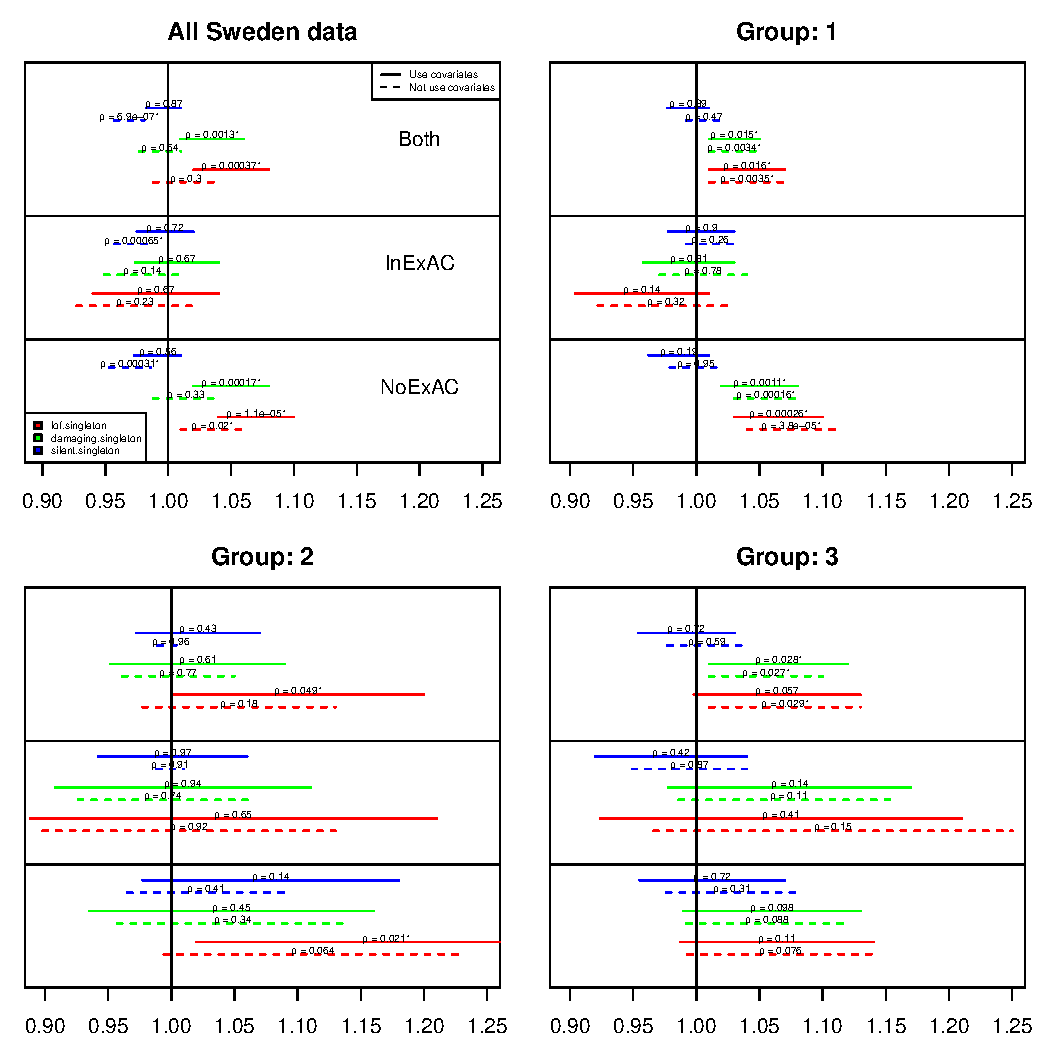
\includegraphics[width=\textwidth, height=8cm]{Picture/ClusteringSwdenPops.pdf}
\caption{Odds ratios for the analysis of all case-control
  samples. Top left picture shows odds ratios for all Sweden samples
  while the three other pictures show odds ratios for three groups
  after the clustering process. Only group 1 and 3 are used in the
  current analysis because there are strong differences between results
  using covariates and not using covariates in group 2. P values were
  calculated for variants in (InExAC), not in (NoExAC) the ExAC database, and all variants (Both).}
\label{fig:homegeneouspopfrompca}
\end{figure}

%%%%%%%%%%%%%%%%%
\subsubsection{Integrated analysis of de novo mutations and
  case-control variants}

Three categories of de novo mutations and two categories of case/control variants were used in the integration analysis process. They included LoF, MiD and silentCFPK denovo mutations; and LoF and MiD case-control variants. We only used MiD and LoF
variants from case-control data. In addition, these variants also
showed similar enrichment in our current analysis as shown in Figure \ref{fig:homegeneouspopfrompca};
therefore MiD and LoF case-control variants were pooled in order to
maximize the case-control information. There were four populations in total. The four populations comprise one de novo population and three
case-control populations: two from the clustering process of the Sweden data and the data from the UK10K project.

\texttt{extTADA} automatically estimated all genetic parameters of SCZ based on the
current data set. All chains showed convergences (Figure \ref{fig:tracePlotMCMCforSCZ}). The proportion of risk genes was approximately
$8.01\%$ (CI = (4.59$\%$, 12.9$\%$)). Regarding de novo classes, LoF had the
highest mean RR, which was 12.25 with CI = (4.78, 22.22). Two other
de novo classes had approximate mean RRs: 1.22 (CI = (1, 2.16)) and
1.44 (CI = (1, 3.16)) for silentCFPK and MiD respectively. For MiD+LoF case-control variants, two Sweden populations had
nearly equal values of mean RRs: 2.09 (CI = 1.04, 3.54)) and 2.44 (CI = 1.04, 5.73)) respectively; however the signal was weak for the
UK population with mean RR only approximately 1.04 (CI = 1, 1.19), (Table \ref{tab:sczResults}, Figure \ref{fig:heatmapSCZ}).


FDRs of genes were also reported by \texttt{extTADA}. There were only four genes (SETD1A, TAF13, PRRC2A, RB1CC1) having
FDR $<$ 0.1 (Table \ref{tab:extTADAforCombinedSCZ}). Both SETD1A (FDR = 0.0033) and TAF13 (FDR = 0.026) showed
individually significant genes. SETD1A had been
confirmed as the highest statistically significant gene of SCZ in previous studies \citep{singh2016rare,
  takata2016novo} while TAF13 was only reported as a potential risk
gene in the study of \cite{fromer2014novo}. Interestingly for the
RB1CC1 gene, rare
duplications were reported to be associated with SCZ with very high
odds ratio (8.58) in the study of \cite{degenhardt2013duplications},
but has not been reported in other studies since. In addition, as
discussed by the authors, duplications at this gene were also observed
by \cite{cooper2011copy} with an odds ratio = 5.29 in a study of 15,767 children with
ID and/or DD.

If we increased the FDR threshold to 0.3 as in the previous ASD study of \citet{de2014synaptic}, there were 13 genes (SETD1A, TAF13, RB1CC1, PRRC2A, VPS13C, MKI67, RARG, ITSN1, KIAA1109, DARC, URB2, HSPA8, KLHL17, ST3GAL6, SHANK1, EPHA5, LPHN2, NIPBL, KDM5B, TNRC18, ARFGEF1, MIF, HIST1H1E, BLNK) which were significant with this threshold. Of these genes, EPHA5, KDM5B and ARFGEF1 did not have any de novo mutations (Table \ref{tab:extTADAforCombinedSCZ}).



\begin{table}[H]
\begin{tabular}{l|r|r|r}
\hline
Parameter & Estimated mode & lCI & uCI \\
\hline
SCZ\_pi0 ($\%$) & 8.01 & 4.59  & 12.9 \\
SCZ\_meanRR\_silentCFPKdenovo & 1.22 & 1.00 & 2.16 \\
SCZ\_meanRR\_MiDdenovo & 1.44 & 1.00 & 3.16 \\
SCZ\_meanRR\_LoFdenovo & 12.25 & 4.79 & 22.22 \\
SCZ\_meanRR\_MiD+LoFccPop1 & 2.09 & 1.04 & 3.54 \\
SCZ\_meanRR\_MiD+LoFccPop2 & 2.44 & 1.05 & 5.73 \\
SCZ\_meanRR\_MiD+LoFccPop3 & 1.04 & 1 & 1.19 \\

\hline
ASD\_pi0 ($\%$) & 4.59 & 3.19 & 6.01 \\
ASD\_meanRR\_MiDdenovo & 3.67 & 1.98 & 8.68 \\
ASD\_meanRR\_LoFdenovo & 23.4 & 13.63 & 36.94 \\
ASD\_meanRR\_LoFcc & 4.18 & 2.04 & 9.96 \\
\hline
ID\_pi0 ($\%$) & 2.76 & 2.07 & 3.7 \\
ID\_meanRR\_MiDdenovo & 28.61 & 16.18 & 41.86 \\
ID\_meanRR\_LoFdenovo & 96.04 & 67.57 & 130.73 \\
\hline
EPI\_pi0 ($\%$) & 1.65 & 0.8 & 3.21 \\
EPI\_meanRR\_MiDdenovo & 47.5 & 19.77 & 87.32 \\
EPI\_meanRR\_LoFdenovo & 77 & 37.19 & 138.24 \\
\hline
DD\_pi0 ($\%$) & 2.87 & 2.34 & 3.49 \\
DD\_meanRR\_MiDdenovo & 22.55 & 13.19 & 32.53 \\
DD\_meanRR\_LoFdenovo & 86.53 & 65.79 & 111.61 \\
\hline

\end{tabular}
\caption{Estimated parameters for de novo and case-control SCZ
  data and four other diseases: ID, EPI, ASD and DD. These results are obtained by sampling 20,000
  times of three MCMC chains. The two last columns show the lower (lCI) and upper (uCI) values of CIs.}
\label{tab:sczResults}
\end{table}

%\subsubsection{TADA results}
%pi = 0.06172522; gDN1 = 17.58647



\begin{figure}[H]
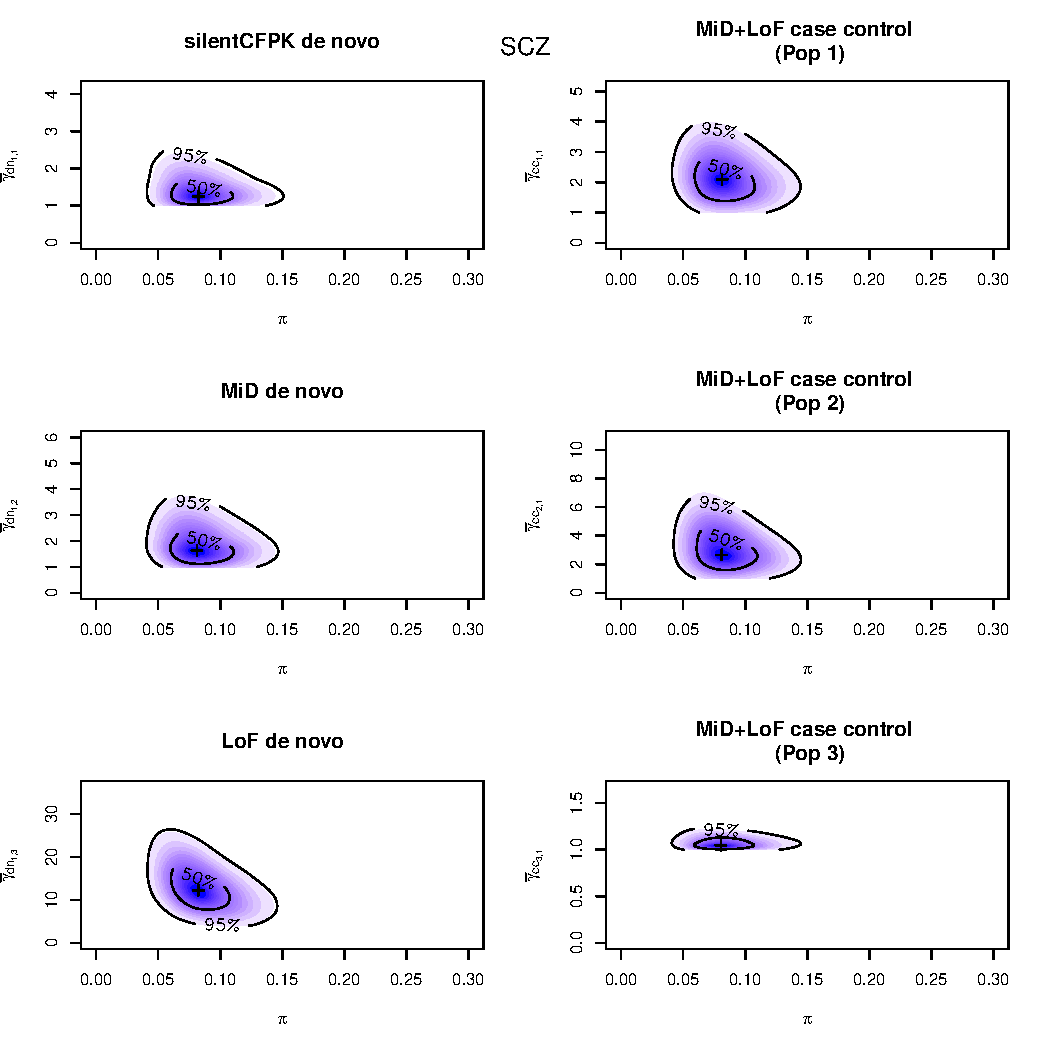
\includegraphics[width=\textwidth,height=8cm]{Picture/HeatMapPostDensitySCZ_combinedCC.pdf}
\caption{The densities of the proportion of risk genes
  and mean relative risks for SCZ data. These are obtained after
  20,000 iterations of three MCMC chains. The first two case-control populations are
  derived from the Sweden data set while the third case-control
  population is the UK population.}
\label{fig:heatmapSCZ}
\end{figure}

\subsubsection{Test enrichment of SCZ-risk genes in gene sets}

From \texttt{extTADA}, we extracted the FDR of each gene and used the information of (1 - FDR) to test the enrichment of gene sets.

\paragraph{Top SCZ significant genes from \texttt{extTADA} are enriched
  in known gene sets}

We first tested 161 known gene sets
(Table \ref{tab:knowngenesetAndAbbreviation}).
Significant results
were observed for 60 gene sets which included gene sets reported by \cite{genovese2016increased}. The most significant gene sets were genes flanking SNPs
and Indels of DD and ASD, missense constrained genes, targets
of fragile X mental retardation protein (FMRP)
genes, loss-of-function intolerant genes (pLI09), RBFOX13, CELF4, CHD8 promoter targets,
RBFOX2, abnormal behavior, abnormal sensory
capabilities$|$reflexes$|$nociception, abnormal motor
capabilities$|$coordination$|$movement, abnormal emotion$|$affect
behavior, abnormal nervous system morphology, ARC (all p $<$ 8.0e-04), Table
\ref{tab:enrichmentGeneSet}). The very significant
result for the abnormal behavior gene set replicated the latest result of
\cite{pardinas2016common}. Furthermore, the gene set obtained from
common variants \citep{pardinas2016common} was also enriched in our
meta-analysis information (p $<$ 5.3e-03). This showed the convergence
(even not very strong in our current study) between
rare-variant and common-variant signal.
The significant results of gene sets of other
neurodevelopmental disorders (NDs: DD, ASD, ID, EPI) showed overlapping
signal between SCZ and these NDs.
In addition, novel results were observed
for essential genes, known epilepsy genes ( p $<$ 1.7e-03, Table
\ref{tab:enrichmentGeneSet}). The essential gene set was just reported
recently by \cite{ji2016increased} as ASD risk genes.


\paragraph{Top SCZ genes are enriched in other gene sets from a
  data-driven approach}

To identify more gene sets enriched in the \texttt{extTADA} results
for SCZ,
we tested 1745 gene sets from different data bases and the 161 gene
sets above. Significant results were observed in 161 gene sets including 36 gene sets in the
 above 161 gene sets (Table \ref{tab:enrichmentGeneSetDataDrivenApproach})
. The top significant gene sets in the known gene sets still had the
lowest p values in these results.

The most interesting result for GO gene
sets was GO:0051179/localization (p = 5.2e-03). This gene set was reported by
\cite{murphy2016bridging} in a study relating to language
evolution and SCZ (Table \ref{tab:enrichmentGeneSetDataDrivenApproach}).

\begin{landscape}
\begin{table}
\small
\begin{tabular}{|l|r|r|l|r|r|}
\hline
Gene set & P value & Adjusted p value & Gene set & P value & Adjusted p value\\
\hline
 DD.allDenovoMiDandLoF & 1e-07 & 2.0e-06 & 	PSD-95\_(core) & 0.0016 & 8.3e-03 \\
celf4 & 1e-07 & 2.0e-06 & 	abnormal\_excitatory\_postsynaptic\_currents & 0.0017 & 8.3e-03 \\
constrained & 1e-07 & 2.0e-06 & 	abnormal\_learning$|$memory$|$conditioning & 0.0017 & 8.3e-03 \\
pLI09 & 1e-07 & 2.0e-06 & 	abnormal\_associative\_learning & 0.0024 & 1.1e-02 \\
rbfox13 & 1e-07 & 2.0e-06 & 	abnormal\_social\_investigation & 0.0027 & 1.2e-02 \\
rbfox2 & 1e-07 & 2.0e-06 & 	abnormal\_synapse\_morphology & 0.0027 & 1.2e-02 \\
FMRP\_targets & 1e-07 & 2.0e-06 & 	abnormal\_neuron\_morphology & 0.0028 & 1.2e-02 \\
abnormal\_behavior & 1e-07 & 2.0e-06 & 	abnormal\_neuron\_physiology & 0.0032 & 1.4e-02 \\
abnormal\_sensory\_capabilities$|$reflexes$|$nociception & 2.2e-06 & 3.9e-05 & 	abnormal\_brain\_morphology & 0.0045 & 1.9e-02 \\
AST.allDenovoMiDandLoF & 2.6e-06 & 4.2e-05 & 	abnormal\_CNS\_synaptic\_transmission & 0.0055 & 2.2e-02 \\
abnormal\_motor\_capabilities$|$coordination$|$movement & 3.2e-06 & 4.7e-05 & 	PSD\_(human\_core) & 0.0064 & 2.5e-02 \\
chd8.human\_brain & 9e-06 & 1.2e-04 & 	abnormal\_aggression-related\_behavior & 0.0073 & 2.8e-02 \\
abnormal\_emotion$|$affect\_behavior & 1.2e-05 & 1.5e-04 & 	abnormal\_brain\_size & 0.0083 & 2.9e-02 \\
abnormal\_nervous\_system\_morphology & 2.7e-05 & 3.1e-04 & 	abnormal\_consumption\_behavior & 0.0084 & 2.9e-02 \\
ARC & 7.5e-05 & 8.0e-04 & 	abnormal\_parental\_behavior & 0.0079 & 2.9e-02 \\
synaptome & 0.00012 & 1.2e-03 & 	abnormal\_spatial\_learning & 0.0081 & 2.9e-02 \\
abnormal\_social$|$conspecific\_interaction & 0.00013 & 1.2e-03 & 	abnormal\_forebrain\_morphology & 0.0093 & 3.2e-02 \\
essentialGenes & 0.00019 & 1.7e-03 & 	abnormal\_innervation & 0.0099 & 3.3e-02 \\
list.EPI.43genes.2017.Epi4K.2017 & 2e-04 & 1.7e-03 & 	abnormal\_response\_to\_new\_environment & 0.013 & 4.2e-02 \\
mir137 & 0.00023 & 1.8e-03 & 	abnormal\_telencephalon\_morphology & 0.013 & 4.2e-02 \\
NMDAR\_network & 0.00023 & 1.8e-03 & 	abnormal\_corpus\_callosum\_morphology & 0.014 & 4.3e-02 \\
mGluR5 & 0.00035 & 2.6e-03 & 	abnormal\_discrimination\_learning & 0.014 & 4.3e-02 \\
abnormal\_fear$|$anxiety-related\_behavior & 0.00061 & 4.2e-03 & 	abnormal\_temporal\_lobe\_morphology & 0.014 & 4.3e-02 \\
abnormal\_cued\_conditioning\_behavior & 0.00062 & 4.2e-03 & 	abnormal\_contextual\_conditioning\_behavior & 0.016 & 4.6e-02 \\
abnormal\_synaptic\_transmission & 0.00069 & 4.4e-03 & 	abnormal\_inhibitory\_postsynaptic\_currents & 0.016 & 4.6e-02 \\
seizures & 0.00072 & 4.5e-03 & 	abnormal\_response\_to\_novelty & 0.016 & 4.6e-02 \\
abnormal\_behavioral\_response\_to\_xenobiotic & 0.00077 & 4.5e-03 & 	abnormal\_brain\_vasculature\_morphology & 0.017 & 4.7e-02 \\
ID.allDenovoMiDandLoF & 0.00079 & 4.5e-03 & 	abnormal\_excitatory\_postsynaptic\_potential & 0.017 & 4.7e-02 \\
Padinas2017\_extTable9.genes & 0.00095 & 5.3e-03 & 	Cav2\_channels & 0.018 & 4.8e-02 \\
ID.allKnownGenes & 0.00099 & 5.3e-03 & 	abnormal\_cerebrum\_morphology & 0.018 & 4.8e-02 \\
\hline
\end{tabular}
\caption{Enrichment of 161 known gene sets from
  \texttt{extTADA} results. These p values were obtained by 10,000,000 simulations, and then adjusted by using the method of \cite{benjamini1995controlling}. The information for these gene sets is
  summarised in Table \ref{tab:knowngenesetAndAbbreviation}.}
\label{tab:enrichmentGeneSet}
\end{table}

\end{landscape}

%%%%%%%%%%%%%%%%%%%%%%%
\subsubsection{Identify number of risk genes for SCZ studies with
  different sample sizes}
We estimated the number of risk genes using the genetic architecture of SCZ inferred from the
current data sets. Different samples sizes (500-20000 and 1000-50000
for families and cases/controls respectively) were simulated. The
number of risk genes with $FDR \le 0.05$ ranged from 0 to 238. Based on
this calculation, we would
expect $> 50$ risk genes if the total sample sizes of families and cases (controls = cases) were
larger than 14,000 (Figure \ref{fig:heatmapcountgenepower}).

\begin{figure}[h]
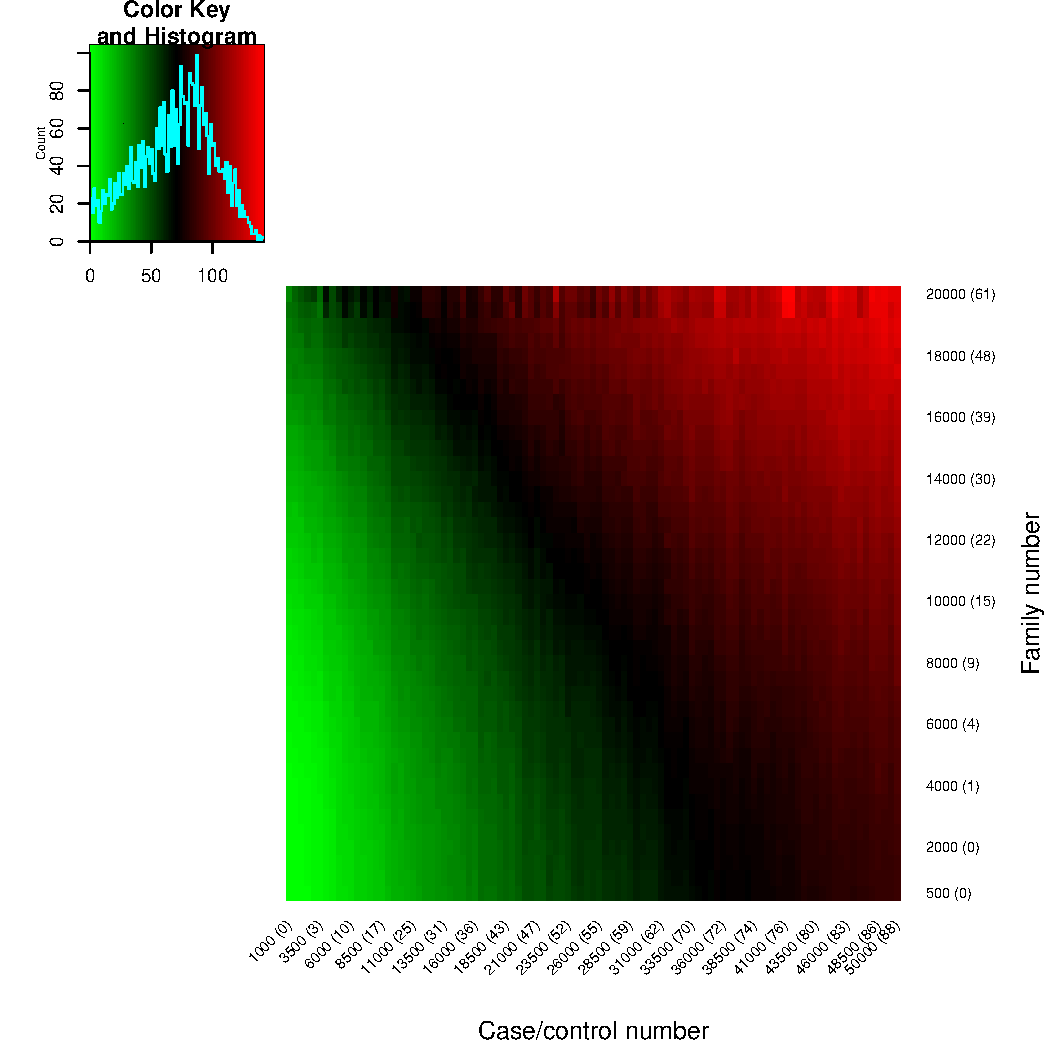
\includegraphics[width=\textwidth,height=8cm]{Picture//heatmap_countgene_powerFDR005.pdf}
\caption{Number of risk genes with different sample sizes based on
  genetic architecture predicted by extTADA. Case/control number is
  only for cases (or controls); therefore if Case/control number =
  10,000 this means total cases+controls = 20,000. The numbers in brackets show risk-gene numbers if we use only case-control data or only de novo mutation data. These results were obtained by resampling 50 times for each combination of sample sizes.}
\label{fig:heatmapcountgenepower}
\end{figure}

%%%%%%%%%%%%%%%%%%%%%
\subsubsection{Test for single classes of SCZ data}

To see the genetic architecture of single classes, and also to test the performance of the pipeline for smaller
number of classes, \texttt{extTADA} was used to estimate parameters separately for four
single classes: only single class of silentCFPK, MiD and LoF de novo
mutations, and only MiD+LoF case-control variants. Overall, the modes of the proportions of risk genes were
less than 8$\%$ and CIs were between 0 to 23.68$\%$ (Table
\ref{tab:SCZgeneticParameterSingleClass}). Regarding the $\pi$ values,
both LoF de novo mutations and MiD+LoF case-control variants showed strong overlapping CIs and
their estimated modes were also not much different: 5.48$\%$ (CI =
(1.24$\%$, $20.62\%$)) and 6.9$\%$ (CI = (2.96$\%$, 13.59$\%$))
respectively. The $\pi$ values of silentCFPK and MiD de novo mutations
were scattered and we also did not see clear convergent results for these
two classes. Mean RRs for these classes were similar to those
estimated using the integrative model above, but their ranges were
large (Table \ref{tab:SCZgeneticParameterSingleClass}). This situation
was similar to what observed in simulated data: using a single category
might result in unreliable results, especially for small mean RRs
(Figure \ref{fig:CCsimulatedDataDetailed}).

%%%%%%%%%%%%%%%%%%%%%%%%%%%%%
\subsubsection{Test genetic architecture of SCZ using both InExAC and
  NoExAC variants}

To see any difference in the genetic architecture of SCZ if all variants
are used, we pooled all InExAC and NoExAC case-control variants and
re-ran \texttt{extTADA} the same way we did as for only NoExAC variants
above. The genetic parameters were similar to NoExAC based results
(Table \ref{tab:SCZgeneticParametersBoth}). However, there were only
three genes with FDR $< 0.1$, even though SETD1A and TAF13 were
still the top significant genes (Table \ref{tab:extTADAforCombinedSCZBoth}).

%%%%%%%%%%%%%%%%%%%%%%%%%%%%%
\subsubsection{Test the influence of mutation rates to the analyzing
  results of SCZ}

The observed counts of silent mutations were lower than expected; therefore,
we multiplied all mutation rates by 0.81 to balance between the observed
and expected counts of synonymous de novo mutations, and then used
\texttt{extTADA} to re-analyze the SCZ data. As expected, genetic parameters
for de novo mutations were slightly higher than in the original analysis;
as a result, the proportion of risk genes also increased to 9.37$\%$
(CI = (5.47$\%$, 15.12$\%$)). Parameters of case-control variants were
not much different (Table
\ref{tab:SCZgeneticParametersAdjustMut}). The most interesting finding was
that the number of significant genes increased to 3 and 6 genes for
FDR $<0.05$ and $<0.1$ respectively. All top significant genes in the
original analysis were among the top genes here (Table \ref{tab:extTADAforCombinedSCZAdjustMut}).


%%%%%%%%%%%%%%%%%%%
%%%%%%%%%%%%%%%%
\subsection{Estimate genetic parameters of other neurodevelopmental diseases using extTADA}

We also used the current pipeline to infer genetic architectures of
ASD, EPI, DD and ID. Sample sizes of these diseases are presented in
Table \ref{tab:alldata}, Figure \ref{fig:wholedataAnalysis}. Overall, except for EPI, the parameter results of the three other
diseases showed strong convergence (Figure
\ref{fig:heatmapotherdiseases}, Table \ref{tab:sczResults}). This
might be because EPI had small family numbers, 392 families compared with $>$
1000 families for other diseases.
The numbers of risk genes ($\pi$) in these diseases were lower
than that of SCZ (Figure \ref{fig:heatmapotherdiseases}, Table \ref{tab:sczResults}).
For ASD, the $95\%$ CI was between
3.19$\%$ and 6.01$\%$ (mode = 4.59$\%$) which overlapped with the result 550-1000 genes estimated in
the original TADA model \citep{he2013integrated} using only LoF de
novo information. For ID, $\pi$ was
smaller than that of ASD; estimated value was 2.76$\%$ (2.1$\%$ to
3.7$\%$ for the 95$\%$ CI). The proportion of risk genes of DD was approximately 2.87$\%$ (CI = c(2.34$\%$, 3.49$\%$) which was similar to that of ID.
The lowest $\pi$ value, $1.65\%$ (95$\%$ CI
= (0.8$\%$, 3.21$\%$)), was observed for EPI. Mean RRs of de
novo mutations in these diseases were much higher than those of
SCZ. This was expected because of the strong signal of de novo mutations
(Table \ref{tab:countAndmutationrate}).
ID, DD had the highest LoF-mutation mean RRs which were 96.04 and
86.53 (CI = (67.57,130.73) and CI = (65.79, 111.6)) respectively. Even though the mean RR of LoF mutations of EPI, which was
77 (CI = (37.19, 138.24)),  was lower
than that of ID; this value for MiD mutations (47.5, CI = (19.77,
87.32)) was much higher than those of other diseases. The mean RR of
EPI had previously been estimated by \cite{phenome2013novo}. Their
result was = 81 which was in the CI of our current results.
For ASD, mean RRs for
de novo mutations were much lower than for these other diseases (Figure
\ref{fig:heatmapotherdiseases}, Table \ref{tab:sczResults}).


\begin{figure}[H]
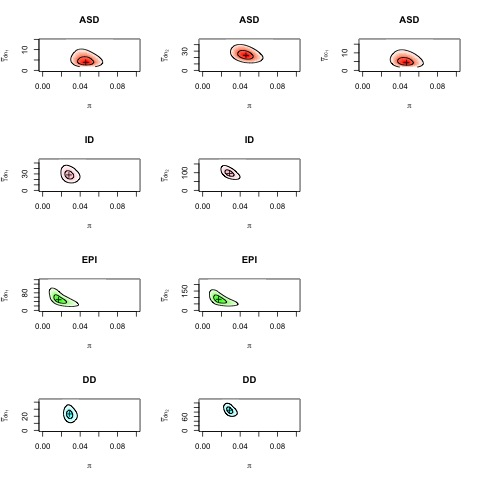
\includegraphics[width=\textwidth,height=14cm]{Picture/HeatMapPostDensityAUTandIDandEPIandDD.jpg}
\caption{The densities of the proportion of risk genes
  and $\pi$ mean relative risks ($\gamma$) for ASD, EPI, ID and DD data. For ASD, there
  are two de novo (dn) classes and one case-control (cc) class. For other
  diseases, only two de novo classes are publicly available for our
  current study.}
\label{fig:heatmapotherdiseases}
\end{figure}

\subsection{Novel risk genes in ID and DD diseases.}

The results of de novo mutations for ID and DD have been
recently reported by using other statistical methods \citep{mcrae2016prevalence, lelieveld2016meta}; therefore, we
aimed to use \texttt{extTADA} to identify novel statistically significant genes from these two
latest data sets. The results of \texttt{extTADA} for these diseases are shown
in Table \ref{tab:extTADAforCombinedID},
\ref{tab:extTADAforCombinedDD}. Genes with FDR $\le$ 0.05 were extracted for the two
diseases. There were 58 and 164 genes for ID and DD respectively. For
 the ID disease, 15/58 genes
 (TCF7L2, USP7, ATP8A1, FBXO11, KDM2B, MED12L, MAST1, MFN1, TNPO2,
 CLTC, CEP85L, AGO1, AGO2, SLC6A1-AS1, POU3F3)
 were not on the list of known ID
 genes as well as 10 significant genes reported by \cite{lelieveld2016meta}. Of the 15
 genes, 6 genes (FBXO11, MFN1,  TNPO2, CLTC,  CEP85L, AGO2) were very significant (FDR $<$ 0.01).
The total MiD and LoF de novo counts of these 15 genes were
 only between 1 and 3. This might be the reason that they were not
 reported as significant genes in the recent study of \cite{lelieveld2016meta}.
Regarding the DD, from the 164 discovered genes, only 59 genes were in
the list reported by \cite{mcrae2016prevalence} while 101 genes were
novel. Similar to ID, the total MiD+LoF de novo counts of these 101 genes were
not high (between 2 and 6). Surprisingly, there were 58 of the 101 genes with
FDRs $<0.01$.


%%%%%%%%%%%%%%%%%%%%%%%%%%%%
%%%%%%%%%%%%%%%%%%%%%%%%
\section{Discussion}

In this work, we have built an integrative pipeline (extTADA) between
case-control variants and de novo mutations to infer genetic
architecture for schizophrenia and four other neurodevelopmental
disorders. The pipeline is based on our previous work for autism studies (TADA).
Even though \texttt{extTADA} is based on TADA, it is a more flexible pipeline.
It is using another strategy to
obtain genetic parameters. \texttt{extTADA} uses the information of
all classes of variants to obtain genetic information which is
different from \cite{he2013integrated} and  \cite{de2014synaptic} in
which LoF de novo mutations play an important role to obtain genetic
information. Using a MCMC method, \texttt{extTADA} estimates all mean
relative risks and the proportion of risk genes simultaneously without
using any previous risk gene sets or prior information (Figure
\ref{fig:wholedataAnalysis}). We are
assuming that different variant classes have similar proportions
of risk genes in a large population, based on some
convergent results between de novo mutations and case-control rare
variants in SCZ \citep{fromer2014novo, purcell2014polygenic,
  singh2016rare}. One important point is that \texttt{extTADA} is able to use for multiple populations. It divides the data into separate small populations and
combines the information across these populations. This is an
advantage of the new pipeline compared with TADA because sequencing
data are usually from different countries/centers. In our current
work, we are using \texttt{extTADA} to apply for the multi-pop issue of
case-control data; however it can be used for multi-pop issues for
both de novo data and case-control data. All integrative information
is used to test the enrichment of gene sets by using the
FDR results of genes.
Finally, \texttt{extTADA} can be
used as TADA if users have prior information relating to the
architecture of the tested disease.

Current study's results replicate previous studies and supply more
information about SCZ. Firstly, SETD1A is the most significant gene
(FDR $\sim 1.5 \times 10^{-3}$) which was reported by \cite{singh2016rare,
  takata2016novo}. In addition, TAF13 is always a significant gene if we
adjust mutation rates or add InExAC variants. Of the two genes RB1CC1
and PRRC2A with FDR $<0.1$, RB1CC1 was reported as the most significant SCZ gene in a
study of copy-number variation in SCZ
\citep{degenhardt2013duplications}. Secondly, significantly
overlapping results between the top genes in this study and known gene
sets such as constrained, de novo SNPs and INDEL of ASD/DD, FMRP, pLI09 genes
show similar trends as the study of
\cite{genovese2016increased}.  Apart
from those results, many GO gene sets also showed significantly results (Table
\ref{tab:enrichmentGeneSet}). Thirdly, from this study, rare-variant
genetic architecture of SCZ is described in details. It is complex,
and may be more complex than those of ASD, ID, DD and EPI (we
have both case-control and de novo data for SCZ while only de novo for
ID, DD and EPI; therefore the comparison might not totally exact). It can be seen
that the number of risk genes
for the disease ($\sim 8\%$) is higher than those of the four other diseases  (Figure \ref{fig:heatmapSCZ} and
\ref{fig:heatmapotherdiseases}, Table \ref{tab:sczResults}). Except
for LoF de novo mutations, mean RRs of case-control variants were
slightly larger than those of de novo mutations. One important point
in our current results is that we see the convergence in the
proportion of risk genes between the LoF de novo mutations and
case-control variants (Table \ref{tab:SCZgeneticParameterSingleClass}). Based on this information and SCZ case/control rare variants have been shown enrichment in genes containing SCZ de novo mutations \citep{genovese2016increased,purcell2014polygenic}, this shows that the SCZ-gene information
is highly overlapping between disruptive de novo mutations and case-control variants. We may probably see a similar trend for the two other classes of de novo mutations if family numbers are large. Finally, we
also see that adding InExAC variants for case/control data do not
improve the prediction results (Table
\ref{tab:SCZgeneticParametersBoth}, \ref{tab:extTADAforCombinedSCZBoth}).

Integrating multiple classes to infer genetic parameters can obtain
more reliable information. As can be seen in our current work, it was
easier to obtain convergent results if multiple classes are integrated
into the estimation process, but the results for single classes do not
show very strong converges in SCZ (Figure \ref{fig:heatmapSCZ},
\ref{fig:tracePlotMCMCforSCZ}, Table
\ref{tab:SCZgeneticParameterSingleClass}), and also in simulation data
(Figure \ref{fig:CCsimulatedDataDetailed}, \ref{fig:2CCsimulatedData}). This
situation is very important because \texttt{extTADA} (and also TADA) is developed for
rare variants. Counts are not high in these
classes of variants; therefore using information from multiple sources
may result in more reliable results. As can be seen in Figure
\ref{tab:CorrelationOneClassCC} and \ref{tab:CorrelationTwoClassCC},
, and \ref{fig:2CCsimulatedData} the information from multiple classes can help obtain more accurate
results especially in cases of small effect sizes.
We do not compare the results of
the current pipeline and TADA on SCZ because \texttt{extTADA} uses all available
information (all classes) while TADA uses specific class/classes
(e.g., LoF variants) to obtain genetic parameters for the disease. In
addition, TADA requires prior information from known gene sets;
however, there is not specific gene sets for SCZ.

The pipeline can be applied to other diseases to obtain genetic
parameters as well as to identify novel significant genes. As be seen in the current study, we are able to use \texttt{extTADA} to infer
genetic parameters for four other neurodevelopmental diseases ASD, EPI, DD and ID (Table
\ref{tab:sczResults}, Figure \ref{fig:heatmapotherdiseases}). The ASD
results of \texttt{extTADA} are comparable with those of \cite{he2013integrated, de2014synaptic}, even though no risk-gene set
was used as prior information in the current estimation process. Regarding the
mean RR of LoF mutations of EPI, the result of \cite{phenome2014novo}
($\sim$ 86) is in the current CI and approximate to the estimated
value of our study (Table \ref{tab:sczResults}). In addition, many
novel significant genes which were missed in recent studies are
discovered by \texttt{extTADA} (101 for DD and 15 for DD).


Apart from that, genetic
architecture can be distinct between classes; for example, recently,
\cite{sifrim2016distinct} have shown some evidence for this hypothesis for de novo
protein-truncating variants (PTVs) and inherited PTVs in congenital
heart defects (CHDs). Therefore, \texttt{extTADA} can be flexibly used to
infer genetic architecture of any specific classes or combining
multiple classes together (e.g., only case-control/inherited variants,
only de novo mutations, or LoF or MiD variants), and can be applied to
other diseases as we did for intellectual disorder, epilepsy,
developmental disorder and autism spectrum disorder in this
study. However, count information should be high in order to obtain
reliable results if only some classes are used.


There are limits in the current SCZ study. Firstly, the model is
developed to use for the combination of non heterogeneous populations. This causes the case-control
sample size smaller after the process of population adjustment. Even
though we are assuming that there are not differences between populations
for de novo data and do not adjust (similar to previous studies
of \cite{de2014synaptic, he2013integrated, singh2016rare}), the
differentiation between populations might happen in this type of
data. Secondly, compared with four other diseases, SCZ de novo counts
are small (Table \ref{tab:countAndmutationrate}) while SCZ family
size is not large in this study (1,077 families). Therefore, the de novo signal is probably not
comparable with that of case-control signal (Table
\ref{tab:SCZgeneticParameterSingleClass}). Finally, we are assuming
that de novo mutations and case-control variants are convergent to the
same proportion of risk genes. We can definitely see different
proportions of risk genes if single class is used in the estimation
process because of sample collections, noise of data. If the
assumption is violated then the current results may probably not
totally reflect genetic architecture of SCZ. However, with overlapping
results between de novo mutations and case-control rare variants
reported recently in SCZ
\citep{purcell2014polygenic,fromer2014novo,genovese2016increased,singh2016rare}
and also in the current study between LoF de novo mutations and MiD+LoF
case/control variants (Table \ref{tab:SCZgeneticParameterSingleClass}), this assumption can be reliable.






\section{Data and methods}

A workflow of all data used in this study is described in Figure \ref{fig:wholedataAnalysis}.

\subsection{Data}

\subsubsection{Simulation data}

The simulation method described in the TADA paper
\citep{he2013integrated} was used to simulate only one case-control
(CC) class, two CC classes and  a combination between one CC and one de novo (DN) class. Different mean RRs and
risk-gene proportions were used in this process.

\subsubsection{Variant data of SCZ, ID, DD, EPI and ASD}

%\normalsize

High-quality variants were obtained from original analyses as
described in Table \ref{tab:alldata}.
Variants were annotated using Plink/Seq (using RefSeq gene
transcripts, UCSC Genome Browser,  http://genome.ucsc.edu) as described in
\cite{fromer2014novo}.
After that, SnpSift version 4.2 \citep{cingolani2012program} was used
to further annotate these variants using dbnsfp31a
\citep{liu2015dbnsfp}. Variants were groups into different
categories. Loss of function (LoF) class comprised of nonsense,
essential splice, and frameshift variants. Missense damaging (MiD) were defined as
missense by Plink/Seq and damaging by results of all of 7 methods \cite{genovese2016increased} from
dbnsfp31a: SIFT, $Polyphen2\_HDIV$, $Polyphen2\_HVAR$, LRT, PROVEAN,
MutationTaster and MutationAssessor. Recently, \citet{takata2016novo} reported significant results for synonymous mutations in regulatory regions; therefore, this category was also analyzed. To annotate synonymous variants within DNase I hypersensitive sites (DHSs) as \citet{takata2016novo}, the file
\emph{wgEncodeOpenChromDnaseCerebrumfrontalocPk.narrowPeak.gz} was
downloaded from \url{http://hgdownload.cse.ucsc.edu/goldenPath/hg19/encodeDCC/wgEncodeOpenChromDnase/}
on April 20, 2016. After that, BEDTools \citep{quinlan2010bedtools} was used to intersect silent
variants/mutations with the DHSs. Based on analyzing results of
\cite{genovese2016increased} in which significant signal was seen for
singleton variants, only case-control singleton variants were used in this study.

The data from Exome Aggregation Consortium (ExAC) \citep{lek2015analysis} were used
to annotate variants inside ExAC (InExAC or not private) and not inside
ExAC (NoExAC or private). On April 20, 2016, the file \emph{ExAC.r0.3.nonpsych.sites.vcf.gz} was downloaded from
\url{ftp://ftp.broadinstitute.org/pub/ExAC_release/release0.3/subsets/}. After
that, BEDTools was used to obtain variants inside (InExAC) or outside this file (NonExAC).

\subsubsection{Gene sets}


Multiple resources were used to obtain gene sets in our study.
Firstly, we used known gene sets with prior evidence for involvement in
schizophrenia and autism from a variety of sources. Secondly, to
identify possible novel significant gene sets, we collected  genes
sets from available data bases.

\paragraph{Known gene sets}

These gene sets and their abbreviations are presented in Table \ref{tab:knowngenesetAndAbbreviation}.

\begin{itemize}
\item Gene sets were enriched for SCZ ultra rare variants which were
  described detailedly in the study
  of  \cite{genovese2016increased}: missense constrained genes
  (constrained) from \cite{samocha2014framework},
loss-of-function tolerance genes (pLI90) from \cite{lek2015analysis},
%brain expressed genes (fagerberg) from \cite{fagerberg2014analysis},
%genes expressed in neurons from \cite{cahoy2008transcriptome} (cahoy),
RBFOX2 and RBFOX1/3 genes (rbfox2, rbfox13) from \cite{weyn2014hits},
Fragile × mental retardation protein targets genes (fmrp) from \cite{darnell2011fmrp},
CELF4 genes (celf4) from \cite{wagnon2012celf4},
synaptic genes (synaptome) from \cite{pirooznia2012synaptomedb},
microRNA-137 (mir137) from \cite{robinson2015genetic},
PSD-95 complex genes (psd95) from \cite{bayes2011characterization},
ARC and NMDA   receptors (NMDARs) genes from \cite{kirov2012novo},
de novo copy number variants in SCZ, ASD, bipolar as presented in Supplementary
Table 5 of \cite{genovese2016increased}.

\item Promoter targets of CHD8 from \cite{cotney2015autism}.

\item Known ID gene set was from the Sup Table 4 of  \cite{lelieveld2016meta}
   and 10 novel genes reported by  \cite{lelieveld2016meta}.

\item Gene sets from MiD and LoF de novo mutations of ASD, EPI, DD, ID.

\item The essential gene set from the supplementary data set 2 of
  \cite{ji2016increased}.

\item Lists of human accelerated regions (HARs) and primate
  accelerated regions (PARs) \citep{lindblad2011high} were downloaded
  from
  \url{http://www.broadinstitute.org/scientific-community/science/projects/mammals-models/29-mammals-project-supplementary-info}
  on May 11, 2016. The coordinates of these regions were converted to
  hg19 using Liftover tool \citep{kent2002human}. We used a similar
  approach as \cite{xu2015genomic} to obtain genes nearby HARs. Genes
  in regions flanking 100 kb of the HARs/PARs were extracted to use in
  this study.

\item List of known epilepsy genes was obtained from Supplementary
  Table 3 of \cite{phenome2017ultra}.

\item 134 central nervous system (CNS) related gene sets were obtained from
  \cite{pardinas2016common}. Steps which were used to obtain the gene
  sets were described in \cite{pocklington2015novel}.
\item List of common-variant genes was obtained from Extended Table 9
  of \cite{pardinas2016common}.

We finally obtained 161 gene sets from this step after removing
overlapping gene sets between previous studies and the 134 gene sets.

\end{itemize}


\paragraph{Other gene sets}

We also used multiple data sets to identify novel gene sets
overlapping with the current gene sets. All gene sets from GO data
basse \citep{gene2015gene}, and other gene sets collected by The
Molecular Signatures Database (MSigDB) \citep{subramanian2005gene}:
 KEGG, REACTOME and C3: motif gene sets. To increase the power of this
 process, we only used gene sets whole lengths were between 100 to 4995
 genes. Totally, there were 1717 gene sets. These gene sets and the above gene sets above were used in this data-drive approach.

\subsection{Methods}

\normalsize

\subsubsection{\texttt{extTADA} pipeline: analyze de novo, transmission and case-control data}


\paragraph{\texttt{extTADA} for one de novo population and one case/control
  population}

\texttt{extTADA} was summarised in Table \ref{tab:ParameterModelleing}
and Figure \ref{fig:TADAandextTADA} in which $x_d \sim Pois(2N_d\mu$,
$\gamma_{dn}), x_{ca} \sim Pois(qN_1\gamma_{cc})$, $x_{cn} \sim
Pois(qN_0)$ and $\gamma_{dn} \sim Gamma(\bar{\gamma}_{dn}\beta_{dn},
\beta_{dn})$, $\gamma_{cc} \sim Gamma(\bar{\gamma}_{cc}\beta_{cc},
\beta_{cc})$, $q \sim Gamma(\rho, \nu)$.



Let K be the number of categories (e.g., missense, MiD, LoF), $x_i =
(x_{i1}, .., x_{iK})$ be the vector of counts at the $i^{th}$ given
gene. The Bayes Factor for each $j^{th}$ category to test two hypotheses: $H_0: \gamma = 1$ versus $H_1:
\gamma \neq 1$ was:

\begin{equation}
\begin{array}{ll}
B_{ij} & = \frac{P(x_{ij}|H_1)}{P(x_{ij}|H_0)} \\
 & = \frac{\int P(x_{ij}|\gamma, q)P(q|H_1)P(\gamma|H_1) dq d\gamma}{\int P(x_{ij}|\gamma, q)P(q|H_0)P(\gamma|H_0) dq d\gamma} \\
 & \stackrel{Because\; \gamma = 1 for\; H_{0}}{=} \frac{\int P(x_{ij}|\gamma, q)P(q|H_1)P(\gamma|H_1) dq d\gamma}{\int P(x_{ij}| q)P(q|H_0)dq}
\end{array}
\label{eq:bayesfactorij}
\end{equation}

In Equation \ref{eq:bayesfactorij}, $x_{ij} = x_d$ and $x_{ij} =
(x_{ca}, x_{cn})$  for de novo, and  case-control data
respectively. In addition, the integral across $q$ was not used for de
novo data because there was not this parameter in de novo data.

As in \cite{he2013integrated}, the BF for the $i^{th}$ gene for combining all categories was:

\begin{equation}
\begin{array}{ll}
B_{i} & =  \prod \limits_{j=1}^{K} B_{ij} \\
\end{array}
\label{eq:bayesfactors}
\end{equation}




To calculate BFs, hyper parameters in Table \ref{tab:ParameterModelleing} were needed to know in advance.
Let $\phi_{1j}$ and $\phi_{0j}$ be hyperparameters for $H_1$ and $H_0$ respectively.
A mixture model of the two hypotheses was used to infer
parameters using information across the number of tested genes ($m$) as
in Equation \ref{eq:internalModel}.

\begin{equation} \label{eq:internalModel}
\begin{array}{ll}
P(x|\phi_1, \phi_0) & = \prod \limits_{i=1}^{m} \left[ \pi \prod \limits_{j=1}^{K} P(x_{ij}|\phi_{1j}) + (1 - \pi) \prod \limits_{j=1}^{K} P(x_{ij}|\phi_{0j}) \right] \\
\end{array}
\end{equation}


The Equation \ref{eq:internalModel} was calculated across categories as
% * <eli.stahl@mssm.edu> 2016-12-23T20:50:32.673Z:
%
% above, you make it sound like we will do Empirical Bayes like He et al. and then you say we use MCMC to get the parameters. In general, empirical Bayesian calculation of BF from "known" (or estimated) parameters may not be the same as fully Bayesian  calculation of BFs using the posterior distribution of parameters. With our Bayesian analysis using MCMC, we can test this and in fact we show that it is similar.
%
% ^.
described in calculating BFs in Equation \ref{eq:bayesfactors}.
The hyperparameters $\phi_{1j} = (\gamma_{j(dn)}, \gamma_{j(cc)},
\beta_{j(dn)}, \beta_{j(cc)}, \rho_j, \nu_j) $ were estimated using a Markov chain
Monte Carlo (MCMC) method named Hamiltonian Monte Carlo (HMC)
implemented in the \texttt{rstan} package \citep{carpenter2015stan, r323manual}. However, Equation \ref{eq:internalModel} was simplified by removing $q \sim Gamma(\rho, \nu)$ in the estimation process of parameters.

\paragraph{Simplified approximate case/control model}

For case-control (inheritance) data, $\frac{\rho}{\nu}$ represented for mean of $q$, and $\nu$ controlled the
  dispersion of $q$; therefore as in the previous study
  of \cite{de2014synaptic}, $\nu$ was heuristically chosen (in all
  current study, 200 was used) and $\frac{\rho}{\nu} = $ the mean frequency across genes by
  using both case and control data.

The case-control model was deployed as follows:
\begin{equation}
\begin{array}{ll}
P(x_{ca}, x_{cn}|H_j) & = P(x_{ca}|x_{ca} + x_{cn}, H_j) P(x_{ca} + x_{cn}| H_j) \\
\end{array}
\end{equation}

Because of $x_{ca} \sim Pois(N_1 q \gamma_{cc})$ and $x_{cn} \sim
Pois(N_0 q)$, assuming that $x_{ca}$ and $x_{cn}$ were
\textbf{independent}, the case data could be modelled as:

$x_{ca}|x_{ca} + x_{cn}, H_j \sim Binomial(x_{ca} + x_{cn}, \theta|H_j)$

with $\theta|H_1 = \frac{N_1 \gamma_{cc}}{N_1 \gamma_{cc} + N_0}$ and $\theta |H_0 = \frac{N_1}{N_1 + N_0}$

The marginal likelihood was

$P(x_{ca}|x_{ca} + x_{cn}, H_j) = \int P(x_{ca}|x_{ca} + x_{cn}, \gamma_{cc}, H_j) P(\gamma_{cc} | H_j) d \gamma_{cc} $

Based on simulation results, the first part $P(x_{ca}|x_{ca} + x_{cn}, H_j)$ can be used to approximately infer mean RRs ($\bar{\gamma}_{cc}$); therefore only this part was used in the estimation process in Equation \ref{eq:internalModel}.


%%%%%%%%%%%%%%%%%%%%%%%%



\paragraph{Control of the proportion of protective vs risk variants using the mean and
dispersion parameters of relative risks}

If $\bar{\gamma}$ and $\beta$ were small then we would see a high proportion of protective variants.
To control for the proportion of protective variants, we tested the
relationship between $\beta$ and $\bar{\gamma}$. We set this proportion very
low (0.5$\%$) and built a nonlinear relationship for $\beta$ and $\bar{\gamma}$
values as in Equation \ref{eq:nonlinearBetaAndGamma} (Figure
\ref{fig:nonlinearRelationBetaAndGamma}). The \textit{nls} in the
\textit{R} version of 3.3.0 \citep{rteam2016} was used to estimate
a, b and c. These estimated values were $6.83, -1.29$ and $
-0.58$ respectively.

\begin{equation}
\label{eq:nonlinearBetaAndGamma}
\beta = e^{a*\bar{\gamma}^b + c}
\end{equation}



\paragraph{\texttt{extTADA} for multiple populations}

To extend the work for multiple populations,
we used the same approach as the integration of information across categories in one
population. Let $Ndn_{pop}, Cdn$ and $Ncc_{pop}, Ccc$ be the
number of populations, categories for de novo and case-control data respectively. The total Bayes Factor of a given gene was the product of
Bayes Factors of all populations as in Equation
\ref{eq:bayesfactorAllPops1}, and all hyper parameters were estimated
using Equation \ref{eq:internalModel22}.

%%%%%%%%%%%%%%%%%%%%%%%%%%%%%%%%%%%%%%%%%%%%%
\paragraph{Predict the number of risk genes}

BFs of genes were calculated using Equation
\ref{eq:bayesfactorAllPops1}. The original case-control model was used
in this calculation; however, we changed the order of the integral of
parameters to not rely on $q$ because the range of this parameter was
not frequently known in advance (Sup Information
\ref{sec:supInformation}). After that, the BFs were converted to false
discovery rates (FDRs) using the method of \cite{newton2004detecting} as described in \cite{de2014synaptic}. The
number of risk genes could be predicted based on a threshold(s)
defined by users.


\subsubsection{Use simulation data to test model}

To calculate the ability of the model in predicting significant genes,
we simulated multiple combinations between one CC category, two CC
categories, one CC category and DN one category data. For CC data,
the original case-control
model in TADA \citep{he2013integrated} was used to simulate
case-control data and then case-control parameters were estimated using
the approximate model. The frequency of SCZ case-control LoF variants was used to
calculate prior information of $q \sim Gamma(\rho, \nu)$ as described
in Table \ref{tab:ParameterModelleing}. For DN data, we used exactly the
original model of TADA in both the simulation and estimation
process.

Different sample sizes were used. For CC data, to see the
performance of the approximate model, we used four sample sizes: 1092
cases plus 1193 controls, 3157 cases plus 4672 controls, 10000 cases
plus 10000 controls, 20000 cases plus 20000 controls. The first two
sample sizes were exactly the same as the two sample sizes from Sweden
data in current study. The last two sample sizes were used to see
whether the model would be better if sample sizes increased. For DN
and CC data, we used exactly the sample sizes of the largest groups in
our current data sets: family numbers = 1077,
case numbers = 3157 and control numbers = 4672.


To see correlations between simulated and estimated parameters,
the Spearman correlation method \citep{spearman1904proof} was used.
To see the performance of the estimation process of parameters inside
the model, we compared between expected FDRs and observed FDRs (oFDRs).

We defined oFDR for a FDR threshold as
follows. Let $G$ be the set of significant genes under the FDR
threshold, and $n_1$ be the length of $G$. Let $n_2$ be the number of real risk genes (information
from simulated data) inside $G$. oFDR for the FDR threshold was the
ratio of $n_2$ and $n_1$ (oFDR = $n_2/n_1$). Estimated paramters from
\texttt{extTADA} were used in this calculation.

For each combination of simulated parameters, we re-ran 100 times and obtained the medians of
estimated values to use for inferences.

We also used different priors of hyper parameters (e.g., $\bar{\bar{\gamma}},  \bar{\beta}$)) in the simulation process and chose the most reliable
priors corresponding with ranges of $\bar{\gamma}$. Because
$\bar{\beta}$ mainly controled the dispersion of hyper parameters, $\bar{\bar{\gamma}}$ was set equal to 1, and only $\bar{\beta}$ was
tested.


\subsubsection{Calculate mutation rates}

We used the methodology which was based on trinucleotide context,
depth of coverage as described in \cite{fromer2014novo} to obtain
mutation rates (MTs) for different classes. There were genes whole mutation
rates were equal to 0 (0-MT genes). To adjust for this situation for each mutation
class, we calculated the minimum MT of genes having this
value $> 0$, then this minimum value divided by 10 was used as MTs of 0-MT genes.

\subsubsection{Analyze SCZ data}

\paragraph{Obtain non-heterogeneous populations for case-control data
  of SCZ}

The case-control data sets were divided into three big populations:
Finland, United Kingdom and Sweden. For the Sweden population, this
was a large data set and was also sequenced at different centers
\citep{genovese2016increased}, therefore we divided this population as follows.

A simple combination between a clustering process using a multivariate normal
mixture model and a data analyzing
strategy using linear and generalized linear models was used to divide
the Sweden data into non-heterogeneous populations.
\cite{genovese2016increased} recently analyzed all case-control data sets by
adjusting for multiple covariates: genotype gender of individuals (SEX), 20
principal components (PCs), year of birth of individuals (BIRTH), Aligent kit
used in wet-labs (KIT) by using linear regression and generalized
linear regression  models
as in Equation \ref{eq:LMandGLM}. They reported significant results
for NonExAC LoF and MiD variants; therefore, this information was used
in this step.
We defined homogeneous populations as populations which were not much
affected by the covariates. Thus, for the populations, analyzing
results using Equation \ref{eq:LMandGLM} (adjusting covariates)
would not be much different from those results using Equation
\ref{eq:LMandGLMnotAdjustment} (not adjusting covariates). The \texttt{mclust}
package Version 5.2 \citep{fraley1999mclust} which uses a multivariate
normal mixture model was used to divide 11,161
samples (4,929 cases and 6,232 controls) into different
groups. To see all situations of the grouping process, we used
\texttt{mclust} with three strategies on 11,161 samples: grouping all
20 PCs, grouping all 20 PCs and total counts, and grouping only the first three PCs.
The number of groups were set between 2 and 6. For each clustering
time, Equation \ref{eq:LMandGLM} and \ref{eq:LMandGLMnotAdjustment} were used
to calculate p values for each variant category of each group from the
clustering results (p1 and p2 respectively); then, Spearman correlation \citep{spearman1904proof} between p-value results
from the two Equations (cPvalue) was calculated. Next, to filter
reliable results from the clustering process, we set criteria:

\begin{itemize}
\item cPvalue $\ge$ 0.85 and p-values for NonExAC $\le$ 0.005.
\item Ratio p1/p2 from Equation \ref{eq:LMandGLM} and
  \ref{eq:LMandGLMnotAdjustment} had to between 0.1 and 1.
\end{itemize}

From results satisfied the above criteria, we manually chose groups
which had similar results between Equation
\ref{eq:LMandGLMnotAdjustment} and \ref{eq:LMandGLM}.


\begin{equation} \label{eq:LMandGLM}
\begin{array}{ll}
logit(P(SCZ = 1)) \sim count + countAll + sex + birth + kit +
  \sum \limits_{i=1}^{20} PC_i \\
count \sim SCZ + countAll + sex + birth + kit + \sum \limits_{i=1}^{20} PC_i
\end{array}
\end{equation}


\begin{equation} \label{eq:LMandGLMnotAdjustment}
\begin{array}{ll}
SCZ & \sim count \\
count & \sim SCZ
\end{array}
\end{equation}

For the data from the UK10K project
\citep{singh2016rare}, we divided the data into two separate
populations England and Finland, and tested NoExAC variants in these
populations by calculating population-size-adjusted ratios between cases
and controls. The ratios were 0.91 and 0.95 for the UK data.
Regarding the Finland data, the ratio for MiD variants was only 0.41 which were
extremely low. This could be a special case for the population or might
be because of other technical reasons. We did not use this population in
the next stage because it showed a different trend with other populations.

\paragraph{Estimate genetic parameters for SCZ}

De novo mutations and case-control variants from the non-heterogeneous
populations were integratively analyzed. Three de novo classes (MiD,
LoF and silentCFPK mutations) and two case-control classes (MiD and
LoF variants) were used in Equation \ref{eq:internalModel} to obtain
genetic parameters for SCZ. Case-control MiD and LoF variants were
pooled into one class in the estimation process.

\paragraph{Estimate number of risk genes for SCZ}

Based on estimated genetic parameters from the data sets available, the number of risk genes were
predicted as described in the \texttt{extTADA} pipeline above. Different thresholds of FDRs were used to
report their corresponding risk-gene numbers.

%%%%%%%%%%%%%%%%%%%%%%%%%
\paragraph{Test enrichment in known gene sets}

Based on the \texttt{extTADA} results, we tested the enrichment of
gene sets by using gene FDRs as
follows. At each gene, we calculated pFDR = 1 - FDR. For each tested gene set, we calculated the mean of pFDRs
 ($m_0$). After that, we randomly choose gene sets $n$ times (n =
10 millions in this study) from the whole genes and
recalculated the means of pFDRs of the chosen gene sets (vector $m$). The p
value for the gene set was calculated as: $p = \frac{length(m[m > m0])
+ 1}{length(m) + 1}$. To correct for multiple tests, the p
values were adjusted using the method of
\cite{benjamini1995controlling} for all the number of tests.



%%%%%%%%%%%%%%%%%%%%%%
\paragraph{Predict number of risk genes for different sample sizes}

Based on the genetic architecture of SCZ, we predicted the number of
risk genes for the disease. To simplify the calculation, we assumed
that sample sizes of cases and controls were the same and only one de
novo and case-control population. In addition, a
 threshold FDR = 0.05 was used in this process to predict a number of
 individually significant genes. Therefore, a
grid of different simulated counts of family numbers between 500 and
20000 and case/control numbers between 1000 and 50000 were
generated. From these simulated counts, we inferred how many risk
genes with FDR $\le 0.05$.

%%%%%%%%%%%%%%%%%%%%%%%%%%%%%%%%%%%%%%%%%%%
\paragraph{Test for single classes}

To have a general picture of all classes, \texttt{extTADA} was used to test for single classes (LoF/MiD/silentCFPK de
novo mutations, LoF/MiD case-control variants only). All parameters were set as the
integration analysis.

\paragraph{Test genetic architecture of SCZ using both InExAC and
  NoExAC variants}

To test whether InExAC variants could increase (or decrease) the
strength of identifying significant genes, we pooled all InExAC and
NoExAC case-control variants and then used \texttt{extTADA} to analyze this pooled
data set.


\paragraph{Test the influence of mutation rates to the analyzing
  results of SCZ}

The de novo data in current study were from different sources;
therefore, de novo counts could be affected by differences in coverage, technologies.
We therefore tested the analyzing results by adjusting for mutation
rates by using synonymous mutations. We divided the observed counts by
expected counts (= 2 x family numbers * total mutation rates), and
then used this ratio to adjust for all mutation rates. The new
mutation rates and the original data (NoExAC) were re-analyzed using \texttt{extTADA}.


%%%%%%%%%%%%%%%%%%%
\subsubsection{Use \texttt{extTADA} to predict genetic parameters of other  neurodevelopmental diseases}

Use exTADA, we analyzed the integration architecture of genetics for
four other  neurodevelopmental diseases: EPI, ID, DD and ASD. For ASD, genetic
parameters were estimated simultaneously for both de novo and
case-control data. For the three other diseases, the estimation
process was only carried out for de novo data because there were not
rare case-control data publicly available.

\subsubsection{Infer parameters using MCMC results}

The \texttt{rstan} package \citep{carpenter2015stan} was used to run MCMC processes. For
simulation data, 5,000 times and a single chain were used. For real
data, 20,000 times and three independent chains were used. In
addition, for SCZ data we used two steps to obtain final
results. Firstly, 10,000 times were run to obtain
parameters. After that, we used Equation
\ref{eq:nonlinearBetaAndGamma} to calculate $\beta$ values
from estimated mean RRs. Finally, \texttt{extTADA} was re-run 20,000 times on the SCZ data
with calculated $\beta$ values set as constants to re-estimate mean
RRs and the proportions of risk genes. For each MCMC process, a
burning period = a half of total running times was used to assure
that chains did not rely on their initial values. For example, we ran
and removed 2,500 burning times before the 5,000 running times for simulation data.

We just chose 1,000 samples of each chain from MCMC results to do
further analyses. For example, with a chain with 20,000 run times, the step to obtain a sample was 20 run times. For all
estimated parameters from MCMC chains, the convergence of each
parameter was diagnosed using the estimated potential
scale reduction statistic ($\hat{R}$) introduced in \texttt{Stan} \citep{carpenter2015stan}. To produce heatmap plots, modes as well as the credible intervals (CIs) of estimated parameters, the Locfit \citep{loader2007locfit} was used. The mode values were used as our estimated values for other calculations.




%%%%%%%%%%%%%%%%%%%%%%%
\section{Acknowledgements}

Research reported in this paper was supported by the Office of Research Infrastructure of the National Institutes of Health under
award number S10OD018522. The content is solely the responsibility of the authors and does not necessarily represent the official views of
the National Institutes of Health.
%%%%%%%%%%%%%%%%%%%%%%%%%%

\section{Supplementary information}

\setcounter{figure}{0}
\renewcommand{\thefigure}{S\arabic{figure}}



\setcounter{table}{0}
%\renewcommand{\tablename}{S}
\renewcommand{\thetable}{S\arabic{table}}
%%\renewcommand{\thetable}{S\arabic}{table}}

\subsection{Sup Table}
%%%%%%%%%%%%%%%%%%%

%%%%%%%%%%%%
\begin{table}[H]
\begin{tabular}{l|r|r|r|r}
\hline

Parameter & & Q50 & Q5 & Q95 \\
$\pi$ & 0.02 & 0.0224 & 0.0125 & 0.0253\\
& 0.05 & 0.0535 & 0.0351 & 0.0611\\
& 0.09 & 0.0965 & 0.0752 & 0.1063\\
& 0.13 & 0.1381 & 0.11 & 0.149\\
\hline
$\bar{\gamma}_{DN}$ & 5 & 4.265 & 3.5608 & 4.947\\
& 10 & 8.575 & 5.7255 & 10.4417\\
& 15 & 13.23 & 9.9955 & 15.925\\
& 20 & 17.07 & 14.2005 & 20.3087\\
\hline
$\bar{\gamma}_{CC}$ & 1.5 & 1.64 & 1.5938 & 1.7888\\
& 2 & 2.21 & 2.1638 & 2.2662\\
& 2.5 & 2.76 & 2.7138 & 2.8575\\
& 3 & 3.225 & 3.14 & 3.31\\
& 3.5 & 3.675 & 3.5812 & 3.7663\\
\hline
\end{tabular}
\caption{Simulated and estimated values of de novo (DN) and
  case-control (CC). Q50, Q5 and Q95 are for quantile values of 0.5,
  0.05 and 0.95 respectively.}
\label{tab:SimulatedParameterOfDNandCC}
\end{table}

%%%%%%%%%%%%%%%%%%%%%%%%%%%%%%%

\begin{table}[ht]
\small
\begin{tabular}{|p{3.5cm}|l|r|r|r|l|}
\hline
Source & Disease &  DN & DN control &   Case &   Control\\
\hline
\cite{fromer2014novo} & SCZ &  617 &    & & \\
\cite{girard2011increased}  & SCZ &  14 &                      &&\\
\cite{gulsuner2013spatial} & SCZ &        105 &     84         &&\\
\cite{mccarthy2014novo} &  SCZ &       57      &                &&\\
\cite{xu2012novo} & SCZ &      231 & 34                      &&\\
\cite{guipponi2014exome} & SCZ & 53 & && \\
\cite{genovese2016increased} & SCZ & & &              4954/4248
                                             &6239/5865 \\
\cite{singh2016rare} & SCZ & & & 1745/1353 & 6789/4769 \\

\hline
\cite{mcrae2016prevalence} & DD & 4293 & & &  \\
\hline
\cite{phenome2014novo} & EPI & 365 & & &  \\
\hline
\cite{de2012diagnostic} & ID & 100 & & &  \\
\cite{hamdan2014novo} & ID & 41 & & &  \\
\cite{rauch2012range} & ID & 51 & 20 & &  \\
\cite{lelieveld2016meta} & ID & 820 &  & &  \\

\hline
\cite{turner2016denovo} & ASD & 5122 & & & \\
\cite{de2014synaptic} & ASD &  & & 404 & 3654 \\
\cite{iossifov2012novo} & ASD & & 343 & & \\
\cite{o2012sporadic} & ASD & & 50 & & \\
\cite{sanders2012novo} & ASD & & 200 & & \\
\hline

\end{tabular}

\normalsize

\caption{De novo and case/control
  data. For ASD studies, \cite{turner2016denovo} integrated previous
  results in their study; therefore only de novo meta data in this study are shown in the table. In
  addition, for ASD case-control data, only one homogeneous Sweden
  population from \cite{de2014synaptic} was used. For case-control
  data of SCZ, after correcting for the population stratification,
  only 4,248 cases (3,157 + 1,091)  + 5,865 (4,672 + 1,193) controls from \cite{genovese2016increased}
  and 1,353 cases + 4,769 controls from \cite{singh2016rare} are used in this study.}
\label{tab:alldata}
\end{table}

%%%%%%%%%%%%%%%%%%%%%%%%%%%%%%%%%
\begin{table}[H]
\begin{tabular}{l|r|r|r|r}
\hline
Disease & Mutation & Count & Sample size & Mutation count per sample size \\
\hline
SCZ &   silentCFPK & 50 & 1077 & 0.05 \\
   & MiD& 105 & 1077 & 0.1 \\
 &   LoF & 116& 1077 & 0.11 \\
\hline
ASD &   MiD & 620 & 5122 & 0.12 \\
 & LoF & 638 & 5122& 0.12 \\
\hline
ID &   MiD & 222 & 1022 & 0.22 \\
 & LoF & 230 & 1022 & 0.23 \\
\hline
EPI &   MiD & 67 & 356 & 0.19 \\
& LoF & 58 & 356 & 0.16 \\

\hline
DD & MiD &  1056& 4293 & 0.25\\
   & LoF & 1078 & 4293 & 0.25\\
\hline
\end{tabular}
\caption{De novo mutation counts of categories and their mutation
  counts per sample size for schizophrenia (SCZ), autism spectrum disorder
  (ASD), epilepsy (EPI), intellectual disorder (ID) and developmental
  disorder (DD).}
\label{tab:countAndmutationrate}
\end{table}

%%%%%%
\begin{table}[H]
\begin{tabular}{l}
\end{tabular}
\caption{extTADA results of SCZ data.}
\label{tab:extTADAforCombinedSCZ}
\end{table}


\begin{table}[H]
\begin{tabular}{p{6cm}p{4cm}p{4cm}}

\hline
Gene set name & Abbreviation & Author \\
\hline
Missense constrained genes & constrained &
\cite{samocha2014framework} \\
Loss-of-function tolerance genes & pLI90 & \cite{lek2015analysis} \\

RBFOX2 and RBFOX1/3 genes & rbfox2, rbfox13 &  \cite{weyn2014hits} \\
FMRP genes & fmrp &  \cite{darnell2011fmrp} \\
CELF4 genes & celf4 &  \cite{wagnon2012celf4} \\
synaptic genes & synaptome & \cite{pirooznia2012synaptomedb} \\
microRNA-137 & mir137 &  \cite{robinson2015genetic} \\
PSD-95 complex genes & psd95 &  \cite{bayes2011characterization} \\
ARC and NMDA   receptors  genes & nmdarc & \cite{kirov2012novo} \\
Essential genes & essential & \cite{ji2016increased} \\
Human accelerated regions and primate accelerated regions & HARs, PARS &  \cite{lindblad2011high} \\
 Known ID gene sets & IDallKnownGenes &   \cite{lelieveld2016meta} \\
Voltage-gated Calcium Channel Genes & vacc &  \\
CHD8 promoter targets & chd8 hNSC, chd8 hNSC specific, chd8 human brain,
               chd8 hNSC human brain, chd8 hNSC human mouse &  \cite{cotney2015autism} \\
\hline
 De novo copy number variants & & \cite{genovese2016increased} \\
ASD &  CNV.denovo.gain/loss.asd & \\
Bipolar & CNV.denovo.gain/loss.bd & \\
SCZ &  CNV.denovo.gain/loss.scz & \\
\hline

MiD and LoF de novo mutations & & \\
DD & DD.allDenovoMiDandLoF & \\
ASD & ASD.allDenovoMiDandLoF & \\
EPI & EPI.allDenovoMiDandLoF & \\
ID & ID.allDenovoMiDandLoF& \\
\hline


\end{tabular}
\caption{Known gene sets used in this study.}
\label{tab:knowngenesetAndAbbreviation}
\end{table}
%%%%%%%%%%%%%%%%%%%

 %%%%%%%%%%%%%%%%%%%%%%%%%%%

\begin{longtable}{|l|r|r|}

%\begin{tabular}{|l|r|r|}
\hline
Gene set & P value & Adjusted p value \\
\hline
\endhead

 DD.allDenovoMiDandLoF  &  1e-07  &  2.3e-05 \\
celf4  &  1e-07  &  2.3e-05 \\
constrained  &  1e-07  &  2.3e-05 \\
pLI09  &  1e-07  &  2.3e-05 \\
rbfox13  &  1e-07  &  2.3e-05 \\
rbfox2  &  1e-07  &  2.3e-05 \\
FMRP\_targets  &  1e-07  &  2.3e-05 \\
abnormal\_behavior  &  1e-07  &  2.3e-05 \\
GGGAGGRR\_V\$MAZ\_Q6  &  3e-07  &  6.3e-05 \\
abnormal\_sensory\_capabilities$|$reflexes$|$nociception  &  2.2e-06  &  4.1e-04 \\
AST.allDenovoMiDandLoF  &  2.6e-06  &  4.4e-04 \\
abnormal\_motor\_capabilities$|$coordination$|$movement  &  3.2e-06  &  5.0e-04 \\
chd8.human\_brain  &  9e-06  &  1.3e-03 \\
ACAGGGT,MIR-10A,MIR-10B  &  9.9e-06  &  1.3e-03 \\
abnormal\_emotion$|$affect\_behavior  &  1.2e-05  &  1.5e-03 \\
GO:0016043  &  1.4e-05  &  1.6e-03 \\
GO:0045202  &  2.1e-05  &  2.3e-03 \\
GO:0071840  &  2.4e-05  &  2.5e-03 \\
abnormal\_nervous\_system\_morphology  &  2.7e-05  &  2.7e-03 \\
CAGGTG\_V\$E12\_Q6  &  3.3e-05  &  3.1e-03 \\
GO:0008104  &  5.3e-05  &  4.7e-03 \\
GO:0051179  &  6.1e-05  &  5.2e-03 \\
GO:0006996  &  6.7e-05  &  5.5e-03 \\
ARC  &  7.5e-05  &  5.9e-03 \\
GO:0043234  &  7.8e-05  &  5.9e-03 \\
CTTTGT\_V\$LEF1\_Q2  &  9.1e-05  &  6.5e-03 \\
AACTTT\_UNKNOWN  &  9.4e-05  &  6.5e-03 \\
GO:0048519  &  0.00011  &  7.4e-03 \\
synaptome  &  0.00012  &  7.8e-03 \\
abnormal\_social$|$conspecific\_interaction  &  0.00013  &  8.1e-03 \\
GGATTA\_V\$PITX2\_Q2  &  0.00014  &  8.5e-03 \\
KEGG\_AXON\_GUIDANCE  &  0.00017  &  1.0e-02 \\
GO:0043005  &  0.00018  &  1.0e-02 \\
essentialGenes  &  0.00019  &  1.0e-02 \\
list.EPI.43genes.2017.Epi4K.2017  &  2e-04  &  1.0e-02 \\
GO:0045211  &  2e-04  &  1.0e-02 \\
mir137  &  0.00023  &  1.1e-02 \\
NMDAR\_network  &  0.00023  &  1.1e-02 \\
GO:0044456  &  0.00023  &  1.1e-02 \\
GO:0022836  &  0.00027  &  1.2e-02 \\
GO:0022839  &  0.00027  &  1.2e-02 \\
GO:0033036  &  0.00029  &  1.3e-02 \\
GO:0034702  &  0.00029  &  1.3e-02 \\
AATGTGA,MIR-23A,MIR-23B  &  0.00031  &  1.3e-02 \\
GO:0097060  &  0.00032  &  1.3e-02 \\
GO:0044765  &  0.00034  &  1.4e-02 \\
mGluR5  &  0.00035  &  1.4e-02 \\
GO:0015276  &  0.00038  &  1.5e-02 \\
GO:0022834  &  0.00038  &  1.5e-02 \\
GO:0048193  &  0.00041  &  1.5e-02 \\
CTTTGA\_V\$LEF1\_Q2  &  0.00044  &  1.6e-02 \\
GO:0097458  &  0.00049  &  1.8e-02 \\
GO:0019226  &  0.00053  &  1.9e-02 \\
GO:0022892  &  0.00054  &  1.9e-02 \\
GO:0005261  &  0.00058  &  1.9e-02 \\
GO:0008022  &  0.00057  &  1.9e-02 \\
abnormal\_fear$|$anxiety-related\_behavior  &  0.00061  &  2.0e-02 \\
abnormal\_cued\_conditioning\_behavior  &  0.00062  &  2.0e-02 \\
GO:0005215  &  0.00064  &  2.0e-02 \\
GO:0048592  &  0.00063  &  2.0e-02 \\
REACTOME\_TRANSMISSION\_ACROSS\_CHEMICAL\_SYNAPSES  &  0.00065  &  2.0e-02 \\
abnormal\_synaptic\_transmission  &  0.00069  &  2.1e-02 \\
GO:0048523  &  0.00069  &  2.1e-02 \\
seizures  &  0.00072  &  2.1e-02 \\
GO:0035637  &  0.00073  &  2.1e-02 \\
abnormal\_behavioral\_response\_to\_xenobiotic  &  0.00077  &  2.2e-02 \\
ID.allDenovoMiDandLoF  &  0.00079  &  2.2e-02 \\
GO:0007268  &  0.00079  &  2.2e-02 \\
Padinas2017\_extTable9.genes  &  0.00095  &  2.5e-02 \\
GO:0005886  &  0.00094  &  2.5e-02 \\
ID.allKnownGenes  &  0.00099  &  2.6e-02 \\
GO:0000904  &  0.00099  &  2.6e-02 \\
GO:0007399  &  0.001  &  2.6e-02 \\
GO:0006810  &  0.0012  &  3.0e-02 \\
GO:0022612  &  0.0012  &  3.0e-02 \\
GO:0015031  &  0.0013  &  3.2e-02 \\
GO:0016568  &  0.0013  &  3.2e-02 \\
GO:0048589  &  0.0014  &  3.3e-02 \\
GO:0051234  &  0.0014  &  3.3e-02 \\
REACTOME\_NEURONAL\_SYSTEM  &  0.0014  &  3.3e-02 \\
GO:0071944  &  0.0015  &  3.5e-02 \\
PSD-95\_(core)  &  0.0016  &  3.6e-02 \\
GO:0042995  &  0.0016  &  3.6e-02 \\
abnormal\_excitatory\_postsynaptic\_currents  &  0.0017  &  3.7e-02 \\
abnormal\_learning$|$memory$|$conditioning  &  0.0017  &  3.7e-02 \\
GO:0005216  &  0.0017  &  3.7e-02 \\
GO:0007154  &  0.0017  &  3.7e-02 \\
GO:0007267  &  0.0018  &  3.8e-02 \\
GO:0010646  &  0.0018  &  3.8e-02 \\
GO:0023052  &  0.0019  &  3.9e-02 \\
GO:0030662  &  0.0019  &  3.9e-02 \\
GO:0044700  &  0.0019  &  3.9e-02 \\
GO:0000139  &  0.0021  &  4.2e-02 \\
GO:0007519  &  0.0021  &  4.2e-02 \\
GO:0045184  &  0.0021  &  4.2e-02 \\
abnormal\_associative\_learning  &  0.0024  &  4.7e-02 \\
GO:0022838  &  0.0025  &  4.7e-02 \\
GO:0023051  &  0.0025  &  4.7e-02 \\
GO:0048731  &  0.0025  &  4.7e-02 \\
GO:0032991  &  0.0026  &  4.9e-02 \\
abnormal\_social\_investigation  &  0.0027  &  4.9e-02 \\
abnormal\_synapse\_morphology  &  0.0027  &  4.9e-02 \\
GO:0010629  &  0.0027  &  4.9e-02 \\
\hline
%\end{tabular}
%\normalsize
\caption{Enrichment of gene sets from different data bases with SCZ
  genes from \texttt{extTADA} results. These p values were obtained by 10,000,000 simulations, and then adjusted by using the method of \cite{benjamini1995controlling}.}
\label{tab:enrichmentGeneSetDataDrivenApproach}
\end{longtable}

%%%%%%%%%%%%
\begin{table}[H]
\begin{tabular}{|l|l|l|l}
\hline
Parameters & Estimated mode & lCI & uCI \\
\hline
SCZ\_pi\_silentCFPKdn & 0.0056 & 0 & 0.1977\\
SCZ\_hyperGammaMean\_silentCFPKdn & 1.5802 & 1.001 & 21.5139\\
SCZ\_pi\_MiDdn & 0.012 & 0 & 0.2368\\
SCZ\_hyperGammaMean\_MiDdn & 1.7486 & 1 & 17.8548\\
SCZ\_pi\_LoFdn & 0.0548 & 0.0124 & 0.2062\\
SCZ\_hyperGammaMean\_LoFdn & 11.1857 & 3.3973 & 31.3602\\
SCZ\_pi\_MiD+LoFcc & 0.069 & 0.0296 & 0.1359\\
SCZ\_hyperGammaMean\_MiD+LoFcc & 2.0176 & 1.2133 & 5.3694\\
SCZ\_hyperGammaMean\_MiD+LoFcc & 3.2288 & 1.2372 & 17.1478\\
SCZ\_hyperGammaMean\_MiD+LoFcc & 1.0691 & 1.0002 & 2.9574\\
\hline
\end{tabular}
\caption{Genetic parameters for SCZ data if single class is used in
  the analysis.}
\label{tab:SCZgeneticParameterSingleClass}
\end{table}
%%%%%%%%%%%%%
%%%%%%%%%%%%%%%%%%%%%%%%%%%
\begin{table}[H]
\begin{tabular}{|l|l|l|l|}
\hline
Parameters & Estimated mode & lCI & uCI \\
\hline
SCZ\_pi0 & 0.0732 & 0.0306 & 0.1506\\
SCZ\_meanRR\_silentCFPKdenovo & 1.2353 & 1.0021 & 3.6086\\
SCZ\_meanRR\_MiDdenovo & 1.4459 & 1.0008 & 4.7004\\
SCZ\_meanRR\_LoFdenovo & 12.0403 & 4.6136 & 25.8786\\
SCZ\_meanRR\_MiD+LoFccPop1 & 1.5856 & 1.1255 & 4.0881\\
SCZ\_meanRR\_MiD+LoFccPop2 & 1.7361 & 1.0438 & 4.8856\\
SCZ\_meanRR\_MiD+LoFccPop3 & 1.0698 & 1.0001 & 2.9991\\
\hline
\end{tabular}
\caption{SCZ genetic parameters using all variants in and not in ExAC
  database (InExAC + NoExAC).}
\label{tab:SCZgeneticParametersBoth}
\end{table}
%%%%%%%%%%%%%%%%%%%%%
\begin{table}[H]
\begin{tabular}{l}
\end{tabular}
\caption{extTADA results of SCZ data uisng all variants in and not in
  ExAC database (InExAC + NoExAC).}
\label{tab:extTADAforCombinedSCZBoth}
\end{table}
%%%%%%%%%%%%%%%%%%%%%%%%%%%%%%%%%%
\begin{table}[H]
\begin{tabular}{|l|l|l|l|}
\hline
Parameters & Estimated mode & lCI & uCI \\
\hline
SCZ\_pi0 & 0.0937 & 0.0547 & 0.1512\\
SCZ\_meanRR\_silentCFPKdenovo & 1.3068 & 1.0005 & 2.7489\\
SCZ\_meanRR\_MiDdenovo & 2.2246 & 1.0006 & 5.3491\\
SCZ\_meanRR\_LoFdenovo & 15.1491 & 5.8606 & 27.3941\\
SCZ\_meanRR\_MiD+LoFccPop1 & 1.8677 & 1.0374 & 3.0736\\
SCZ\_meanRR\_MiD+LoFccPop2 & 2.2632 & 1.003 & 4.9168\\
SCZ\_meanRR\_MiD+LoFccPop3 & 1.0372 & 1.0002 & 1.1807\\
\hline
\end{tabular}
\caption{SCZ genetic parameters after adjusting mutation rates (NoExAC).}
\label{tab:SCZgeneticParametersAdjustMut}
\end{table}

%%%%%%%%%%%%%%%%%%%%%
\begin{table}[H]
\begin{tabular}{l}
\end{tabular}
\caption{extTADA results of SCZ data after adjusting mutation rates.}
\label{tab:extTADAforCombinedSCZAdjustMut}
\end{table}




%%%%%%%%%%%%%%%%%%%%%
\begin{table}[H]
\begin{tabular}{l}
\end{tabular}
\caption{extTADA results of ID data.}
\label{tab:extTADAforCombinedID}
\end{table}

\begin{table}[H]
\begin{tabular}{l}
\end{tabular}
\caption{extTADA results of DD data.}
\label{tab:extTADAforCombinedDD}
\end{table}

\begin{table}[H]
\begin{tabular}{l}
\end{tabular}
\caption{extTADA results of ASD data.}
\label{tab:extTADAforCombinedASD}
\end{table}

%%%%%%%%%%%%%%%%%%%%%%%%
\subsection{Sup Figure}


\begin{figure}[H]
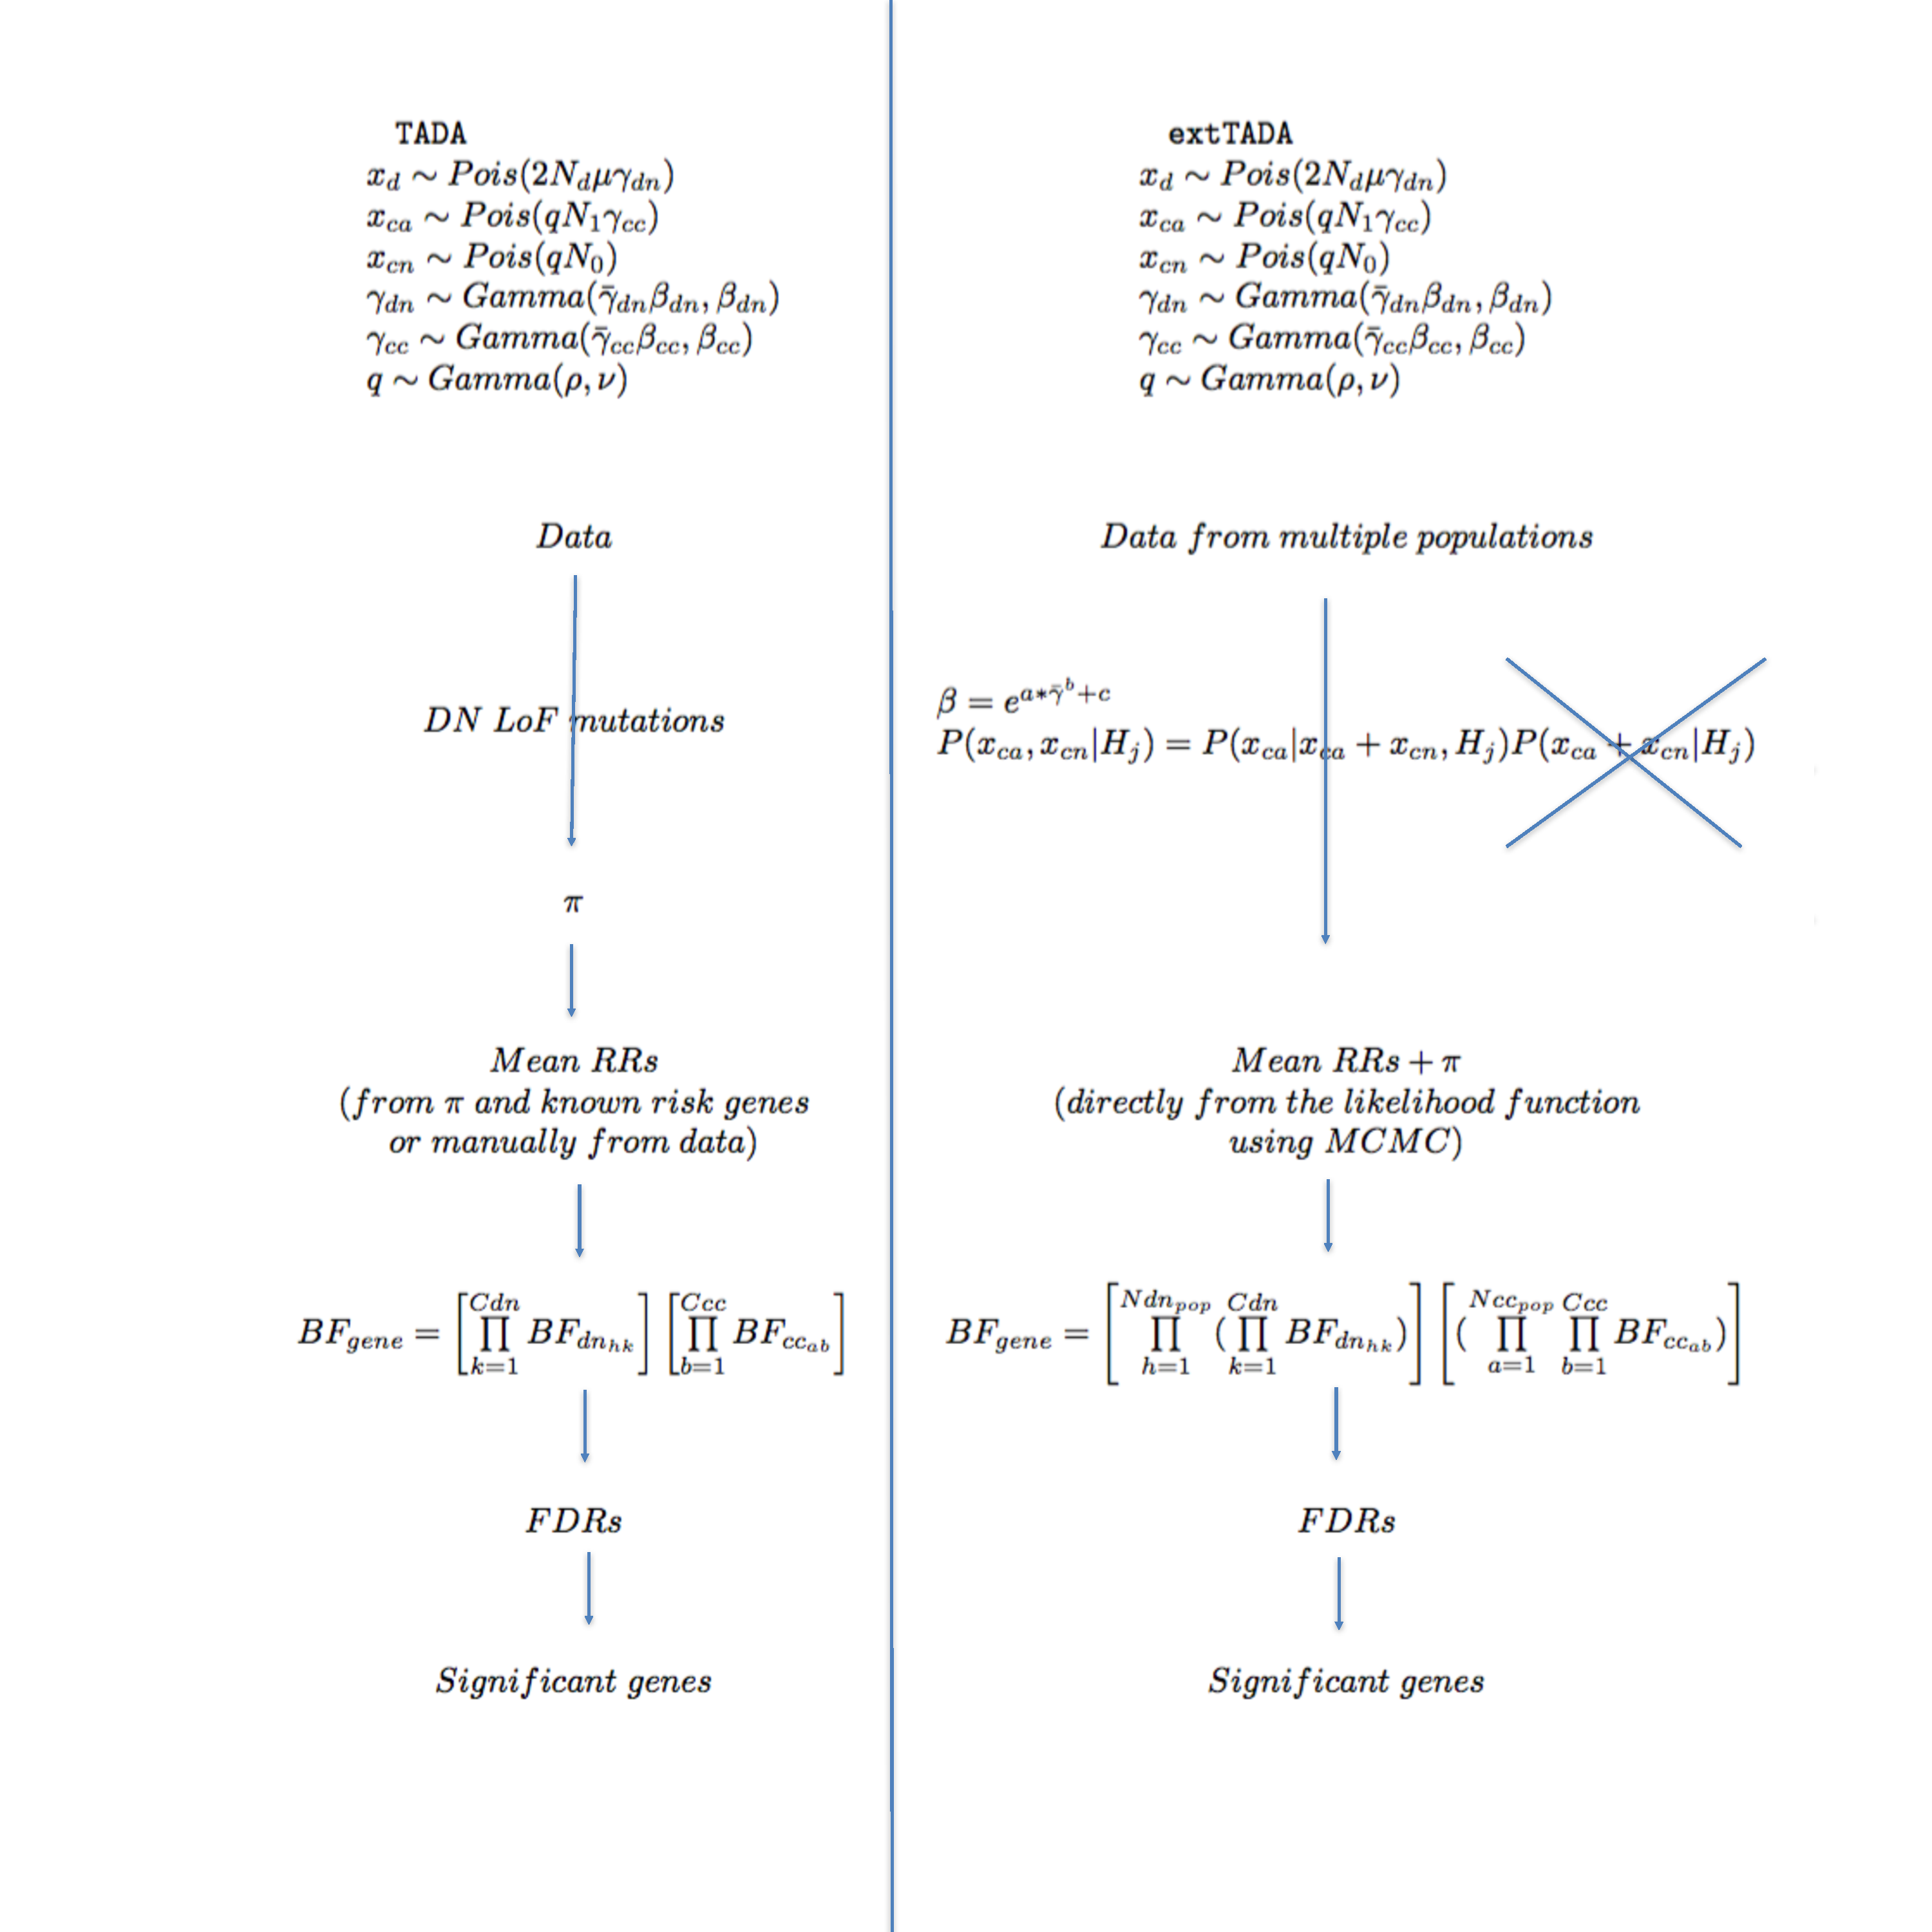
\includegraphics[width=\textwidth,height=\textwidth]{Picture/TADAextTADAcomparison.pdf}
\caption{Comparison between \texttt{TADA} and
  \texttt{extTADA}. They both use the same model for de novo
  data ($x_{dn}$ and case/control ($x_{ca}, x_{cn}$)
  data. \texttt{extTADA} combines all categories to obtain parameters
  while \texttt{TADA} is based on LoF mutations. \texttt{extTADA} uses
  an approximate model for case-control data, and constrains $\beta$
  and $\bar{\gamma}$ in the estimation process. \texttt{extTADA} is
  designed to work for multiple populations. \texttt{TADA} can be used
  inside \texttt{extTADA}.}
\label{fig:TADAandextTADA}
\end{figure}


\begin{figure}[H]
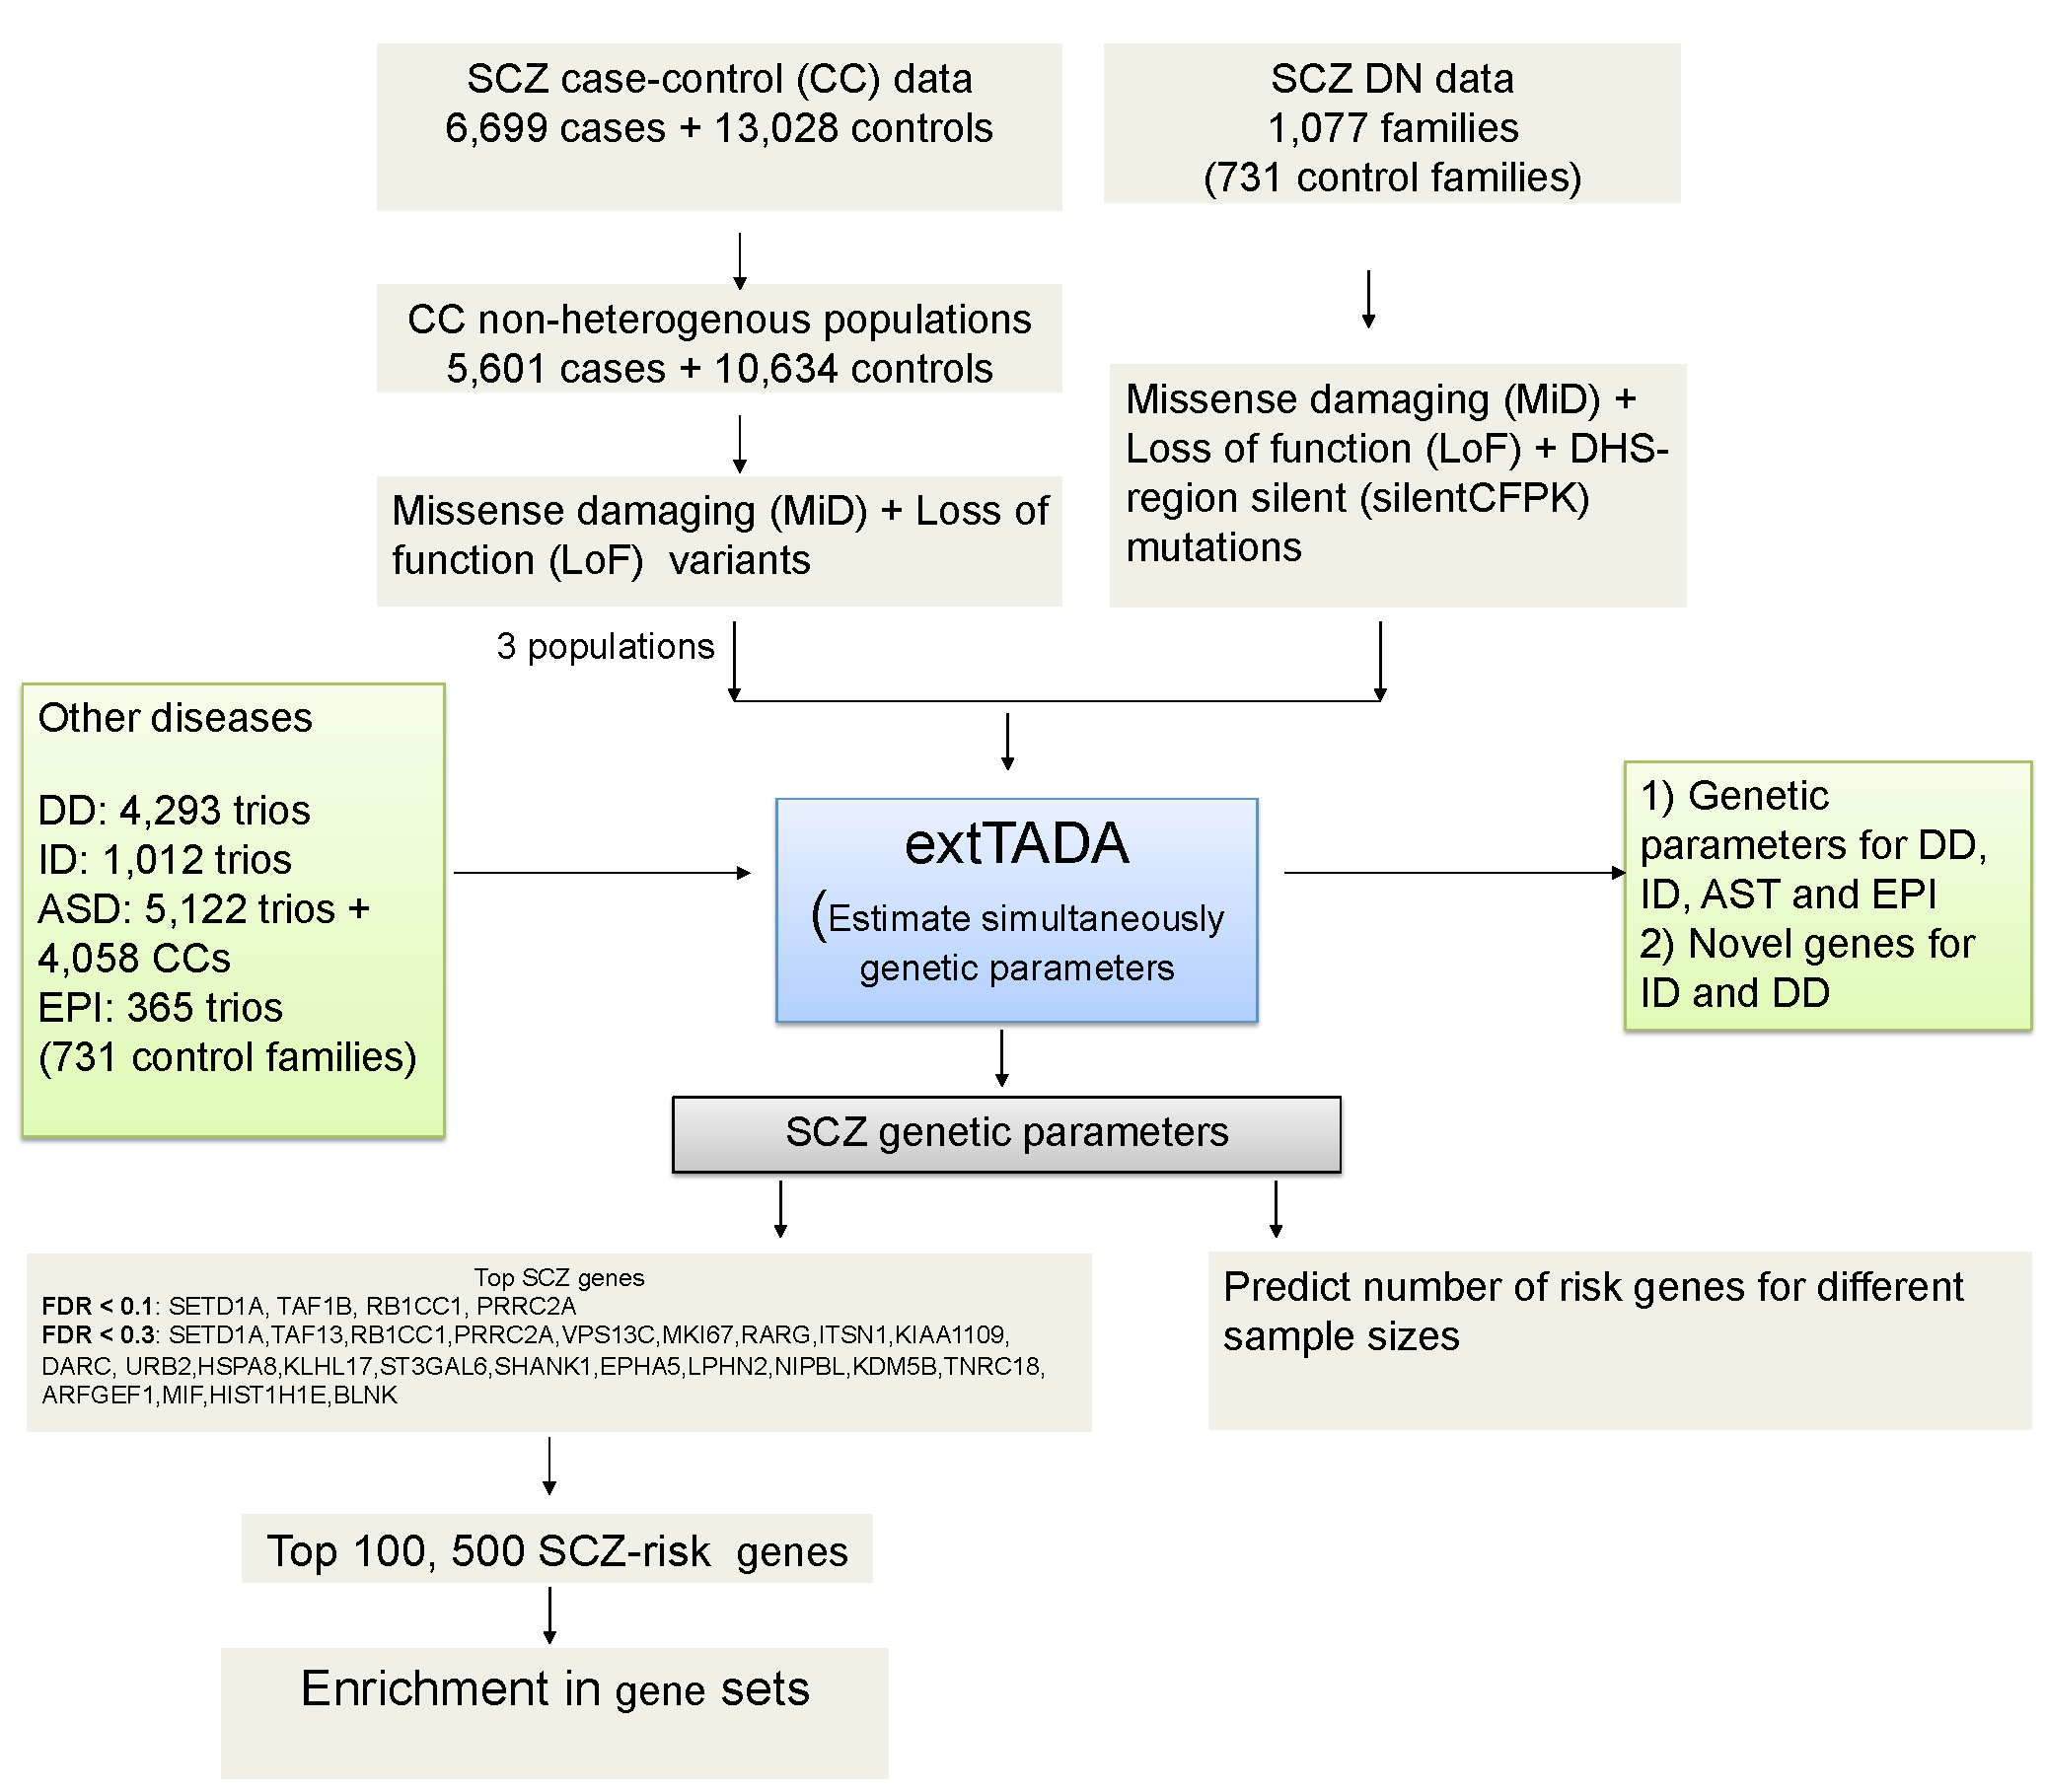
\includegraphics[width=\textwidth,height=\textwidth]{Picture/wholeDataAnalysis.pdf}
\caption{Workflow of data analysis.}
\label{fig:wholedataAnalysis}
\end{figure}



\begin{figure}[H]
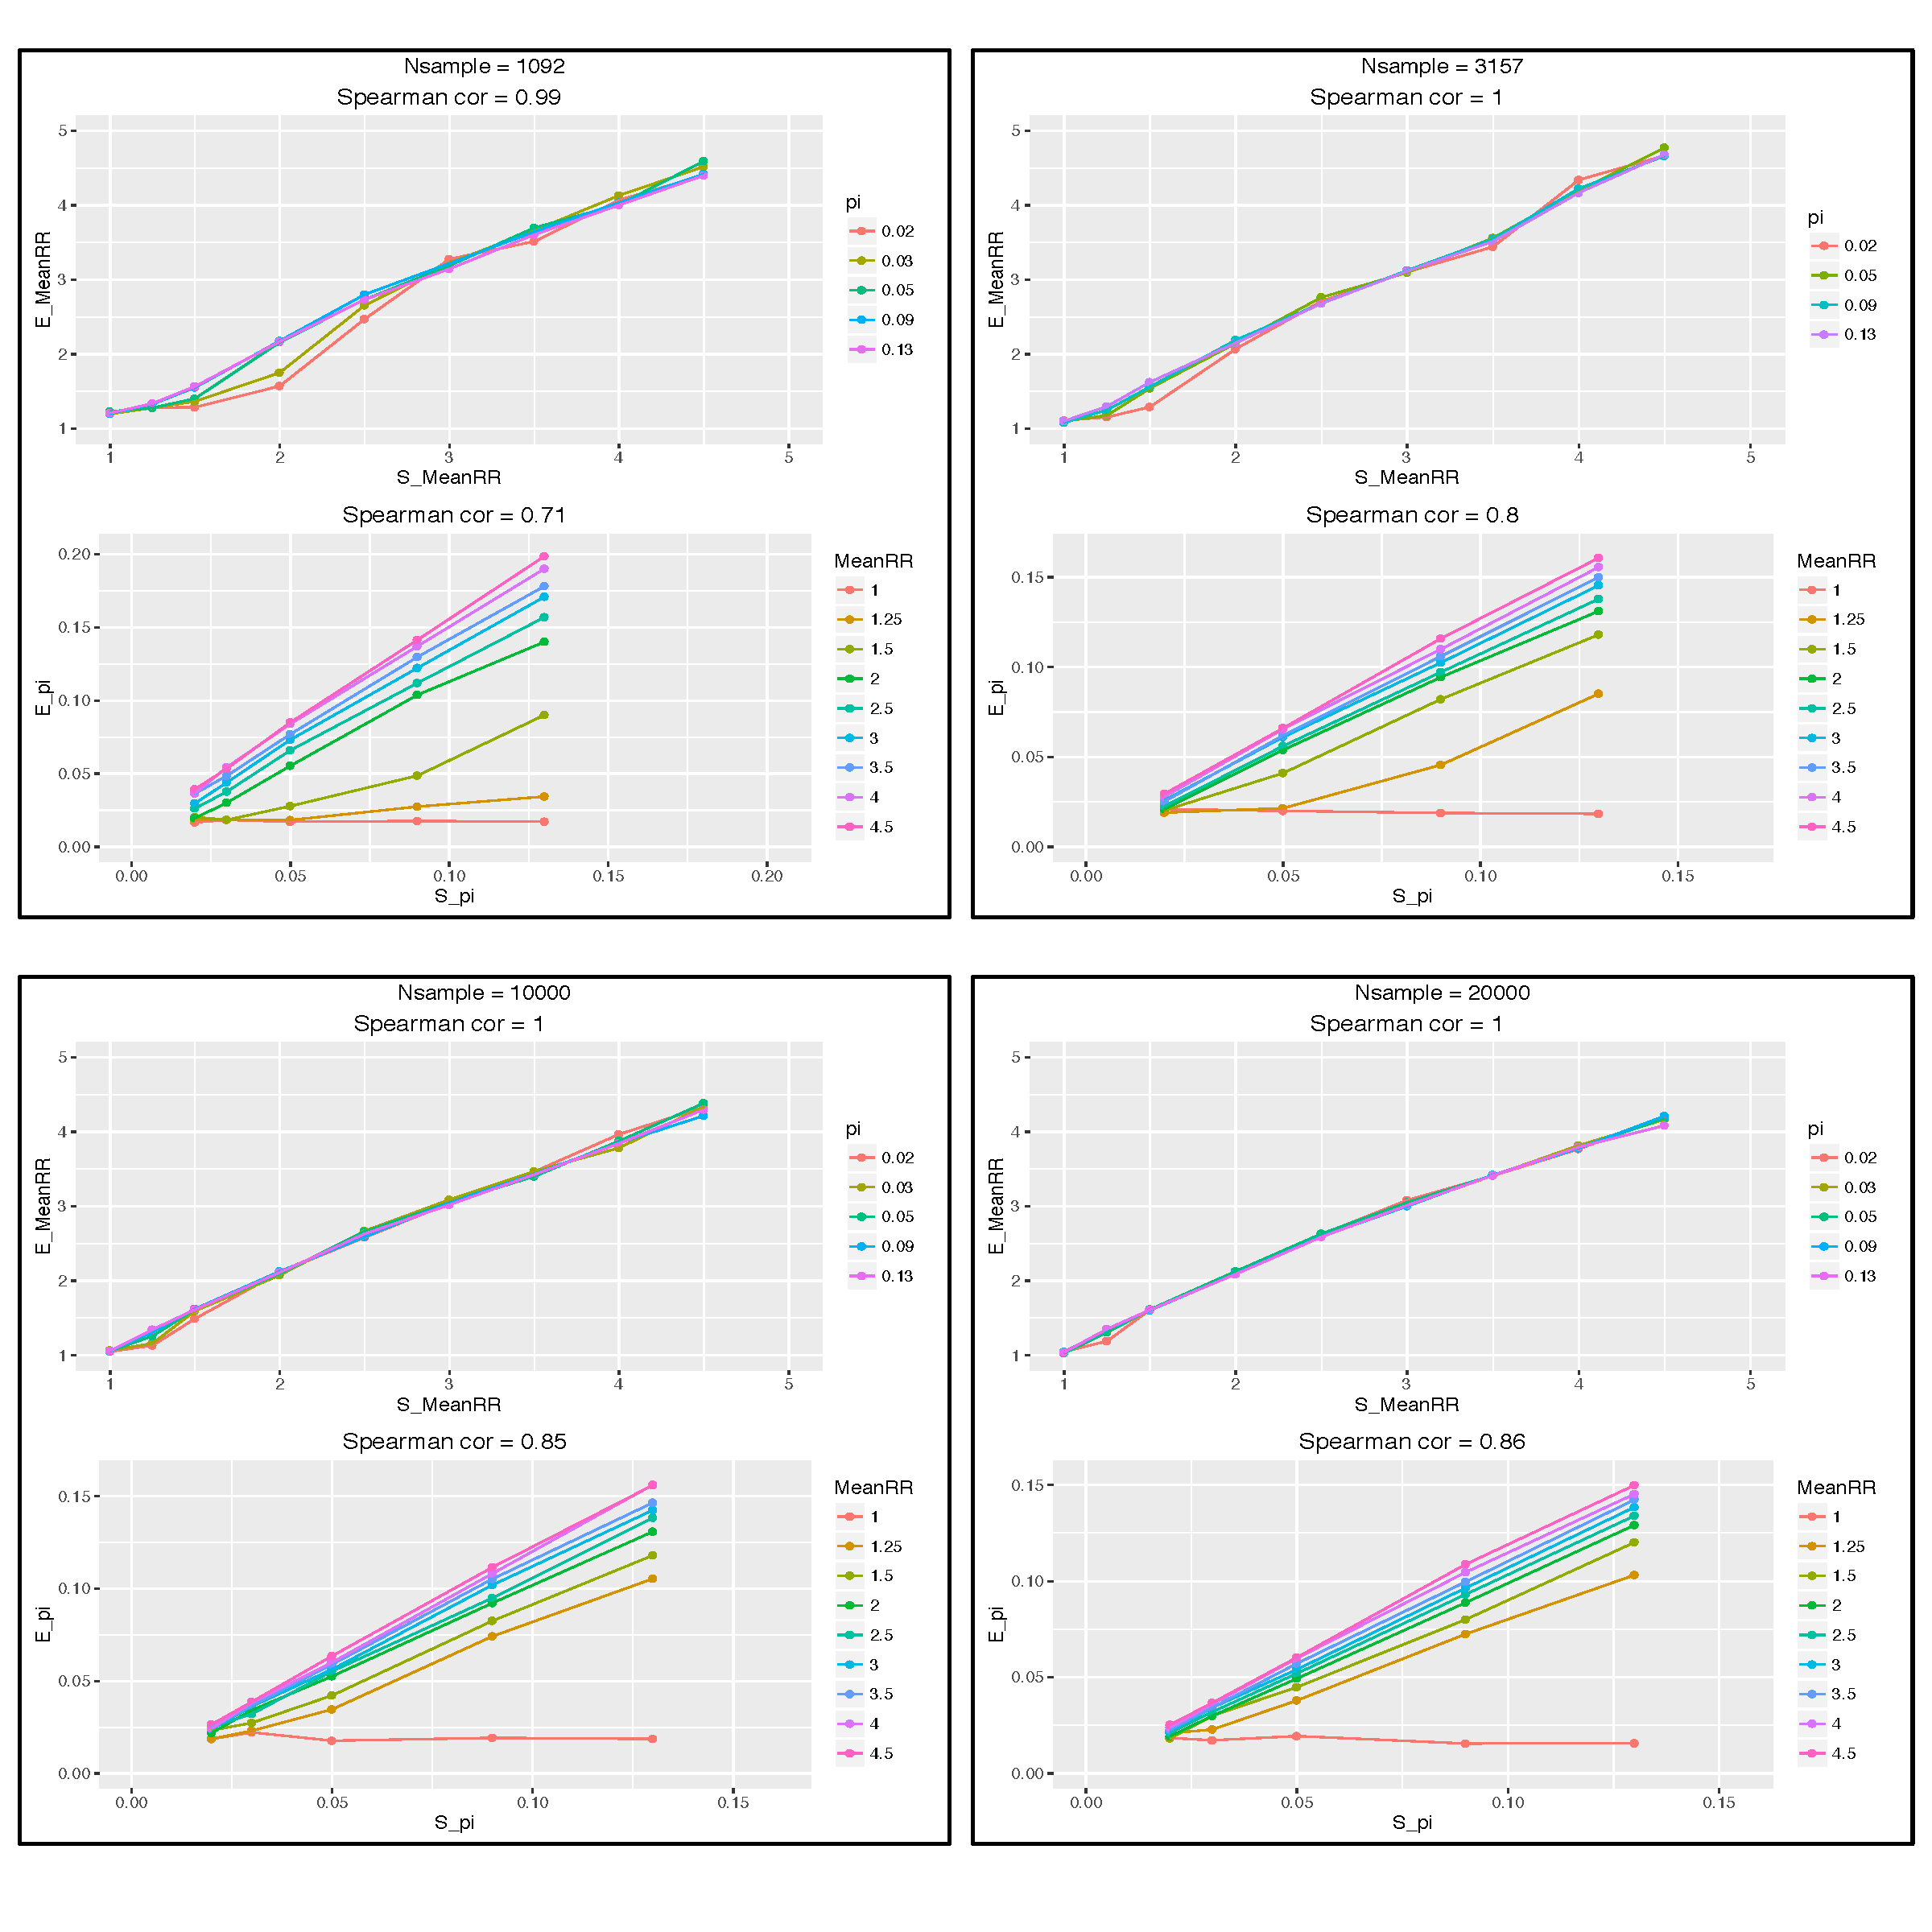
\includegraphics[width=\textwidth,height=\textwidth]{Picture/SimulationOnlyCC.pdf}
\caption{Correlation between simulated and estimated values for
  one-category case/control data.}
\label{fig:CCsimulatedDataDetailed}
\end{figure}

\begin{figure}[H]
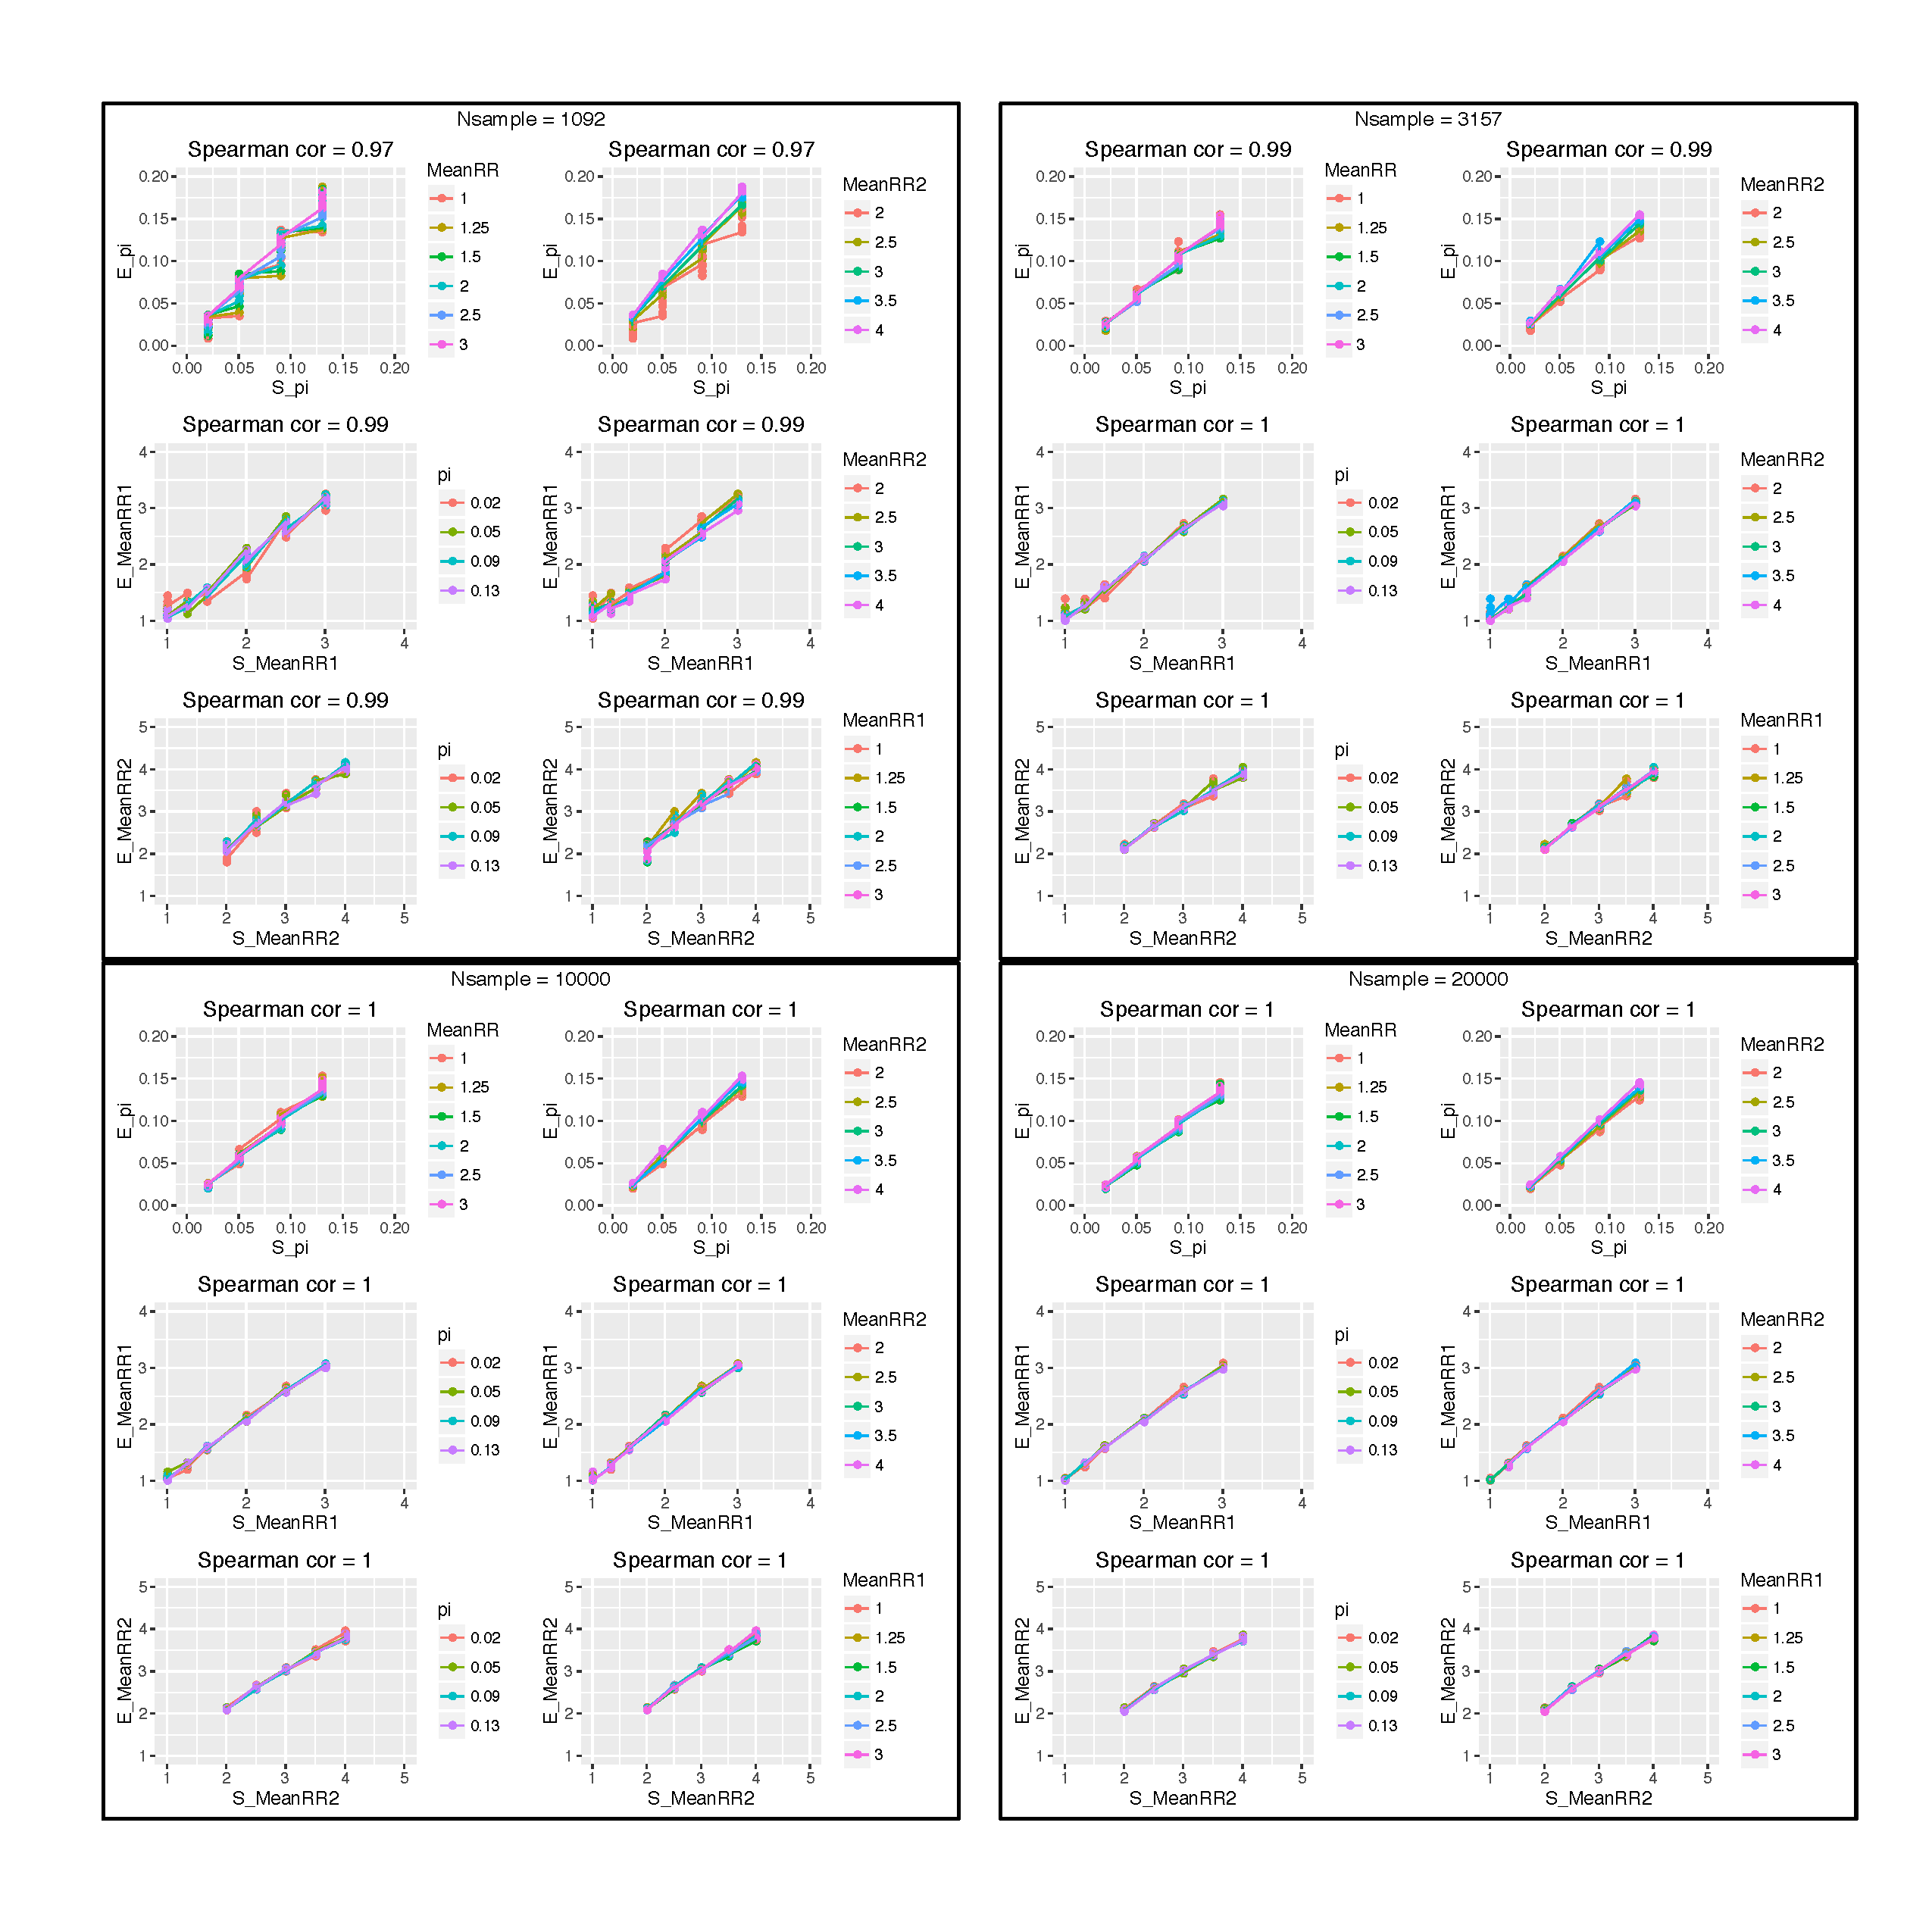
\includegraphics[width=\textwidth,height=\textwidth]{Picture/Simulation2CC.pdf}
\caption{Correlation between simulated and estimated values for
  two-category case/control data.}
\label{fig:2CCsimulatedData}
\end{figure}



\begin{figure}[H]
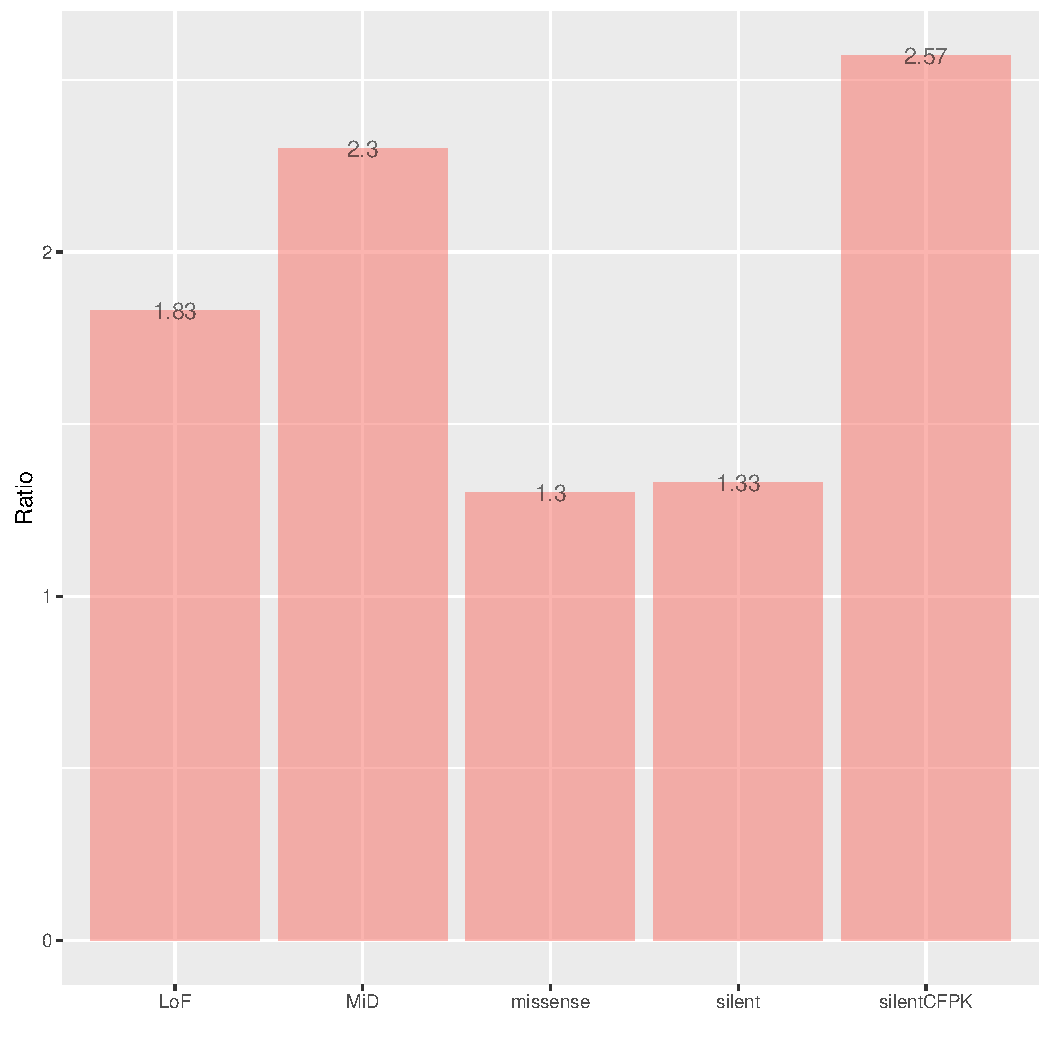
\includegraphics[width=\textwidth,height=\textwidth]{Picture/SCZ_DNcasecontrolRatio.pdf}
\caption{Ratios of de novo mutations between SCZ probands and controls
  (unaffected siblings). "silentCFPK" describes for silent mutations within frontal cortex-derived
  DHS (silentCerebrumfrontalocPk.narrowPeak). MiD mutations are missense mutations derived from
  7 methods. }
\label{tab:denovomutation}
\end{figure}

\begin{figure}[H]
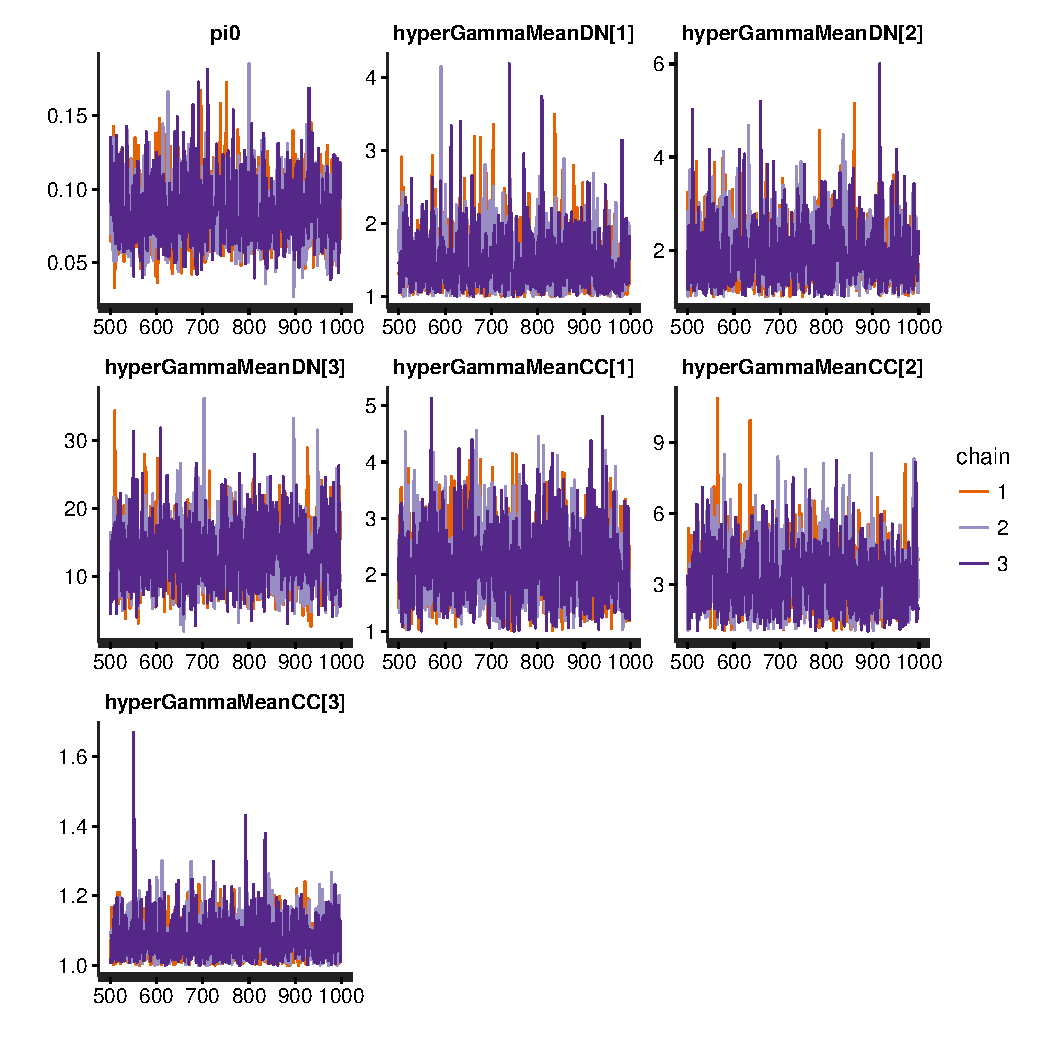
\includegraphics[width=\textwidth,height=8cm]{Picture/MCMCtraceplotSCZ_combinedCC.pdf}
\caption{MCMC results for SCZ data.}
\label{fig:tracePlotMCMCforSCZ}
\end{figure}


\begin{figure}[H]
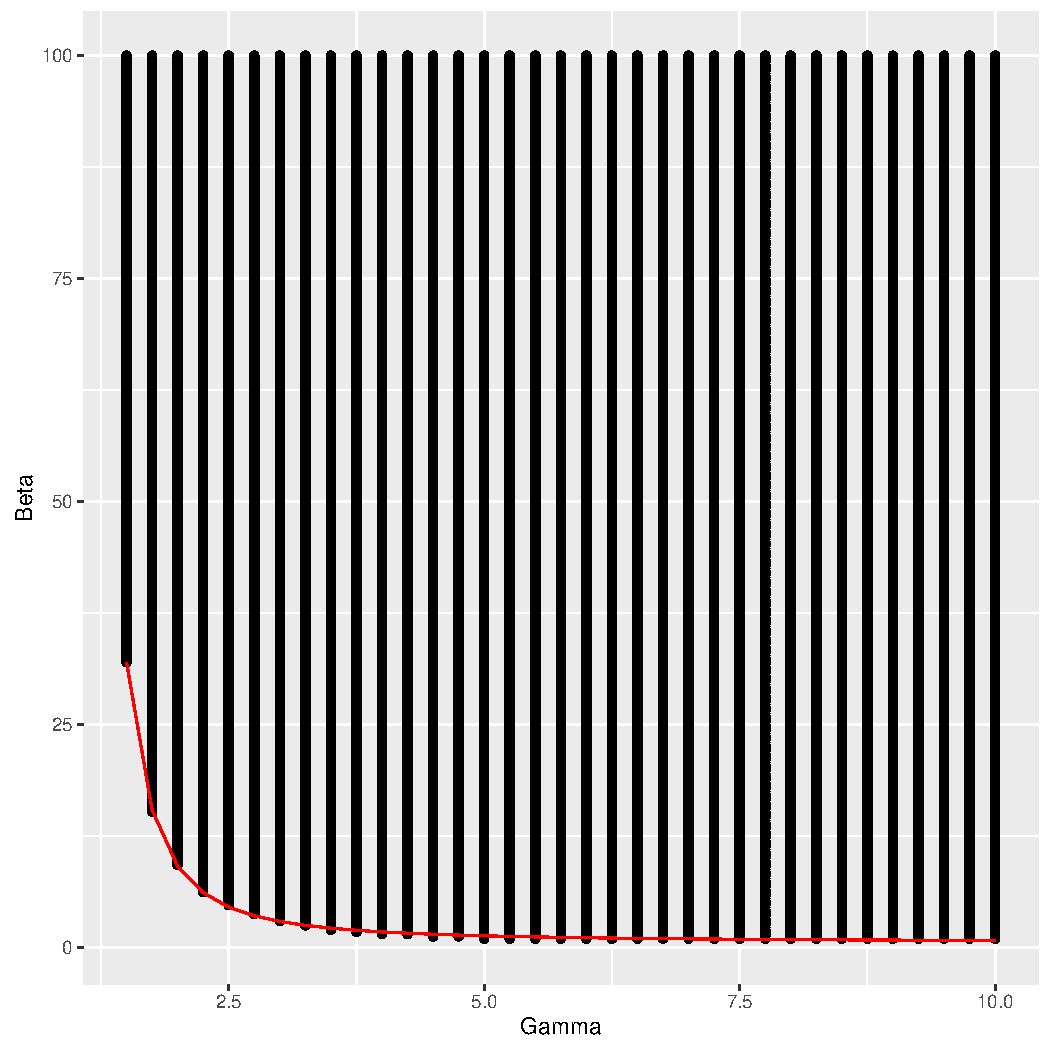
\includegraphics[width=\textwidth, height=8cm]{Picture/BetaAndGammaCorrelation.pdf}
\caption{A grid of $\beta$ and $\gamma$ values. Points on the red line
are corresponding with the proportion of protective variants less than
0.0$\%$.}
\label{fig:nonlinearRelationBetaAndGamma}
\end{figure}




\subsection{Sup Information}
\label{sec:supInformation}

\paragraph{Calculate Bayes Factor for case/control data}

At a given gene, Bayes Factor for each class was calculated as $BF = \frac{P(x_1, x_0|H_1)}{P(x_1, x_0|H_0)}$. The probability for each model ($H_j, j = 0, 1$) was calculated order to rely only $\gamma$ parameters as follows.

\begin{equation}
P(x_{ca}, x_{cn}|H_j) = P(x_{cn}|H_j) P(x_{ca}|x_{cn}, H_j)
\end{equation}
\begin{itemize}
\item The first part $P(x_{cn}|H_j)$ was the same as \cite{de2014synaptic}:
\begin{equation}
P(x_{cn}|H_j) = \int P(x_{cn}|q, H_j) P(q|\rho, \nu, H_j) dq = NegBin(x_{cn}|\rho, \frac{N_0}{\nu + N_0}), j = 0,1
\end{equation}

\item The second part:
\begin{equation} \label{eq:casecontrolNewIntegral}
\begin{array}{ll}
P(x_{ca}|H_j, x_{cn}) & = \int P(x_{ca}|q, \gamma_{cc}) P(q|H_j, x_{cn}) P(\gamma_{cc} |H_j) dq d\gamma_{cc}  \\
& = \int \left[ P(x_{ca}|q, \gamma_{cc}) P(q|H_j, x_{cn}) dq \right] P(\gamma_{cc} |H_j) d\gamma_{cc} \\
& = \int NegBin(x_{ca}|\rho + x_{cn}, \frac{N_0 + \nu}{N_1 \gamma_{cc} + N_0 + \nu}) P(\gamma_{cc} |H_j) d\gamma_{cc}
\end{array}
\end{equation}
\end{itemize}

To identify the lower and upper limits of $\gamma_{CC}$ for the integral, we randomly sampled 10,000 times values from the $Gamma(\bar{\gamma}_{cc} * \beta_{cc}, \beta_{cc})$ and used the minimum and maximum values for the lower and upper limits respectively.

\bibliography{referenceForMainPaper}

\end{document}
